% ============================================================
%  AeroMoE: A Resource-Efficient Collaborative Edge AI System
%            for In-situ Mixture-of-Depths-Experts Inference
%  IEEE Transactions / Conference Format (IEEEtran)
% ============================================================

\documentclass[journal]{IEEEtran}

% ---- packages ------------------------------------------------
\usepackage[T1]{fontenc}
\usepackage[utf8]{inputenc}
\usepackage{cite}
\usepackage{amsmath,amssymb,amsfonts}
\usepackage{algorithmic}
\usepackage{algorithm}
\usepackage{graphicx}
\usepackage{textcomp}
\usepackage{xcolor}
\usepackage{booktabs}
\usepackage{url}
\usepackage{array}
\usepackage{multirow}
\usepackage{tikz}
\usepackage{CJKutf8}

% 2. PDF注释支持
\usepackage{pdfcomment}
% 3. 确保注释使用Unicode编码
\hypersetup{unicode}

% circled number command (used for step annotations)
\newcommand{\circled}[1]{%
  \tikz[baseline=(char.base)]{%
    \node[shape=circle,draw,inner sep=1pt,font=\scriptsize] (char) {#1};}}

% keep long URLs from overflowing
\Urlmuskip=0mu plus 1mu

% ---- hyphenation hints ---------------------------------------
\hyphenation{op-tical net-works semi-conduc-tor Mix-ture-of-Ex-perts}

% ==============================================================
\begin{document}
\begin{CJK*}{UTF8}{gbsn}
\bstctlcite{IEEEexample:BSTcontrol}

% ---- title & authors -----------------------------------------
\title{AeroMoE: A Resource-Efficient Collaborative Aerial Edge AI System for LLM Inference}

% \author{%
%   \IEEEauthorblockN{%
%     Mingyi Dong,
%     Dixiang Gao,
%     Liangliang Fu,
%     Shulei Zeng,
%     Qing Wei,
%     Yao Ge,\\
%     Xiqing Liu,
%     and 
%     Guiling Wang}
%     %\thanks{This work was supported by the National Key Research and Development Program of China under Grant 2020YFB1806703. \emph{(Corresponding authors: Xiqing Liu; Nian Xia.)}} 
%     \thanks{This work was supported in part by NCUT Research Start-up Foundation under Grant 110051360026XN085-28, in part by Beijing Municipal Natural Science Foundation under Grant 4254065, and in part by the National Key R\&D Program of China under Grant 2023YFB2904600. ({\it Corresponding Author: Dixiang Gao.})}
%     \thanks{Mingyi Dong, Dixiang Gao, Qing Wei, and Guiling Wang are with Beijing Key Laboratory of Key Technologies for AI+ Domain Applications, North China University of Technology, Beijing 100144, China (email: {\tt \{mydong, gao.dixiang, weiqing, wangguiling\}@ncut.edu.cn}).}
%     \thanks{Liangliang Fu is with China United Network Communications Co., Ltd. Jiangxi Branch, Nanchang 330096, Jiangxi, China. (email: {\tt  full50@chinaunicom.cn}).}
%     \thanks{Shulei Zeng is with Unicom Research Institute, Beijing 102600, China. (email: {\tt  zengsl15@chinaunicom.cn}).}
%     \thanks{
%     Yao Ge is with the AUMOVIO-NTU Corporate Lab, Nanyang Technological University, Singapore 639798 (e-mail: {\tt yao.ge@ntu.edu.sg}).}
%     \thanks{
%     Xiqing Liu is with the State Key Laboratory of Networking and Switching Technology, School of Information and Communication Engineering, Beijing University of China Posts and Telecommunications, Beijing 100876 (e-mail: {\tt liuxiqing@bupt.edu.cn}).}
%   % \IEEEauthorblockA{\IEEEauthorrefmark{1}%
%   %   School of Computer Science and Engineering,
%   %   Southern Tech University, Guangzhou, China\\
%   %   \{weiliang, linjiahao, tangruoyu, zhanghao\}@stu.edu.cn}
%   % \IEEEauthorblockA{\IEEEauthorrefmark{2}%
%   %   Department of Electrical and Computer Engineering,
%   %   University of Technology, Hong Kong SAR, China\\
%   %   xian.chen@ust-ece.hk}

% }


\maketitle


% ---- abstract ------------------------------------------------
\begin{abstract}
% 混合专家模型（Mixture-of-Experts, MoE）通过为不同任务激活部分专家，为资源受限环境下的高效推理提供了一种可行思路。然而，在 UAV 边缘网络中部署 MoE 模型仍面临多重挑战：UAV 的内存和计算能力有限，UAV 之间的单跳通信链路带宽受限，不同任务对专家的需求分布也具有明显差异。若直接部署所有原始专家，容易超过 UAV 的存储能力；若仅依据专家需求进行部署，则可能忽略专家之间的相似替代关系以及跨 UAV 通信代价。

% 为解决上述问题，本文提出 AeroMoE，一种面向 UAV 边缘推理的相似性感知专家部署与调度方法。AeroMoE 首先根据专家相似度构造可替代专家集合，并将原始专家需求扩展为候选专家的有效需求；随后设计通信感知部署评分，综合考虑专家需求、UAV 连通性、链路速率、计算能力和冗余部署成本。在此基础上，AeroMoE 采用两阶段动态贪心部署策略：预部署阶段优先保证必要专家需求可服务，动态调整阶段在 UAV 内存约束下进一步选择收益较高且冗余较低的专家部署方案。最后，AeroMoE 基于部署结果进行轻量级逐层推理调度，为每个专家执行步骤选择本地或单跳可达的 UAV。

% 仿真实验结果表明，在随机热点 UAV 场景下，AeroMoE 相比 RandomPlacement、Importance 和 No-Sim 分别降低了约 $23.0\%$、$20.4\%$ 和 $48.2\%$ 的平均端到端推理延迟。结果说明，相似专家替代能够缓解 UAV 内存受限下的专家覆盖压力，通信感知部署能够减少不必要的跨 UAV 传输，从而提升资源受限 UAV 边缘网络中的 MoE 协同推理效率。
Mixture-of-Experts (MoE) models enable efficient inference through sparse expert activation. They are attractive for onboard intelligence in unmanned aerial vehicle (UAV) edge networks, where low-latency processing over wide areas is required without reliable cloud connectivity. However, deploying MoE models remains difficult. UAV edge networks feature heterogeneous onboard resources, limited link bandwidth, and spatially heterogeneous task demands. Directly loading the full expert set readily exhausts the limited memory of individual UAVs.
To address this issue, we propose AeroMoE, a similarity-aware framework for collaborative MoE inference. The framework constructs substitutable expert sets based on similarity and extends basic demands into effective demands. It then computes multi-dimensional expert placement scores considering demand, UAV connectivity, communication rate, computing power, and redundancy cost. A two-stage dynamic greedy algorithm decides expert placements on UAVs to ensure critical coverage while balancing gain and redundancy under memory constraints. Finally, a lightweight per-layer scheduler selects the best local or single-hop UAV to execute each {\color{black}expert step}. %\pdfcomment{这个是解决另一个老师的comment：修改：AeroMoE 的目标是在 UAV 资源约束下最小化端到端推理延迟。为此，框架依次完成任务需求建模、可替代专家构造、专家—UAV 部署评分与部署决策，最终为每个专家执行步骤选择本地或单跳可达 UAV，降低通信与计算开销。-----英文版：The goal of AeroMoE is to minimize end-to-end inference latency under the constraints of UAV resources. To this end, the framework successively completes task requirement modeling, alternative expert construction, expert-UAV deployment scoring and deployment decision-making. Finally, for each expert execution step, local or single-hop reachable UAVs are selected to reduce communication and computing overhead.}
Simulations show that AeroMoE reduces average end-to-end inference latency by 24.1\%, 21.1\%, and 48.3\% %\pdfcomment{这几个百分比,没在仿真中点出是哪里提升的}
compared with random placement, importance-based placement, and similarity-agnostic deployment, respectively. These results confirm the effectiveness of similarity-aware substitution and communication-aware placement. AeroMoE offers a practical solution for collaborative intelligence in resource-limited aerial edge networks.
\end{abstract}

\begin{IEEEkeywords}
UAV edge computing, Mixture-of-Experts, expert deployment,
similarity-aware substitution, collaborative inference.
\end{IEEEkeywords}

\IEEEpeerreviewmaketitle

% ==============================================================
\section{Introduction}
\label{sec:intro}
% ==============================================================

% 随着边缘智能的发展，UAV 边缘网络逐渐成为低时延任务处理的重要平台。UAV 可以根据任务区域灵活部署，并通过空中链路为地面用户提供计算与通信服务，适用于应急感知、空中巡检、目标识别和协同监测等场景~\cite{mozaffari2019uav,zhu2019uav}。与此同时，混合专家模型（Mixture-of-Experts, MoE）通过稀疏激活机制仅调用部分专家完成推理，
% 在扩展模型容量的同时降低单次计算开销，因而为资源受限边缘环境中的智能推理提供了新的可能~\cite{shazeer2017moe,fedus2022switch,jiang2024mixtral}。

% 然而，将 MoE 推理直接部署到 UAV 边缘网络中并不简单。首先，UAV 搭载的计算和存储资源有限，难以在每个 UAV 上部署完整专家集合；当专家数量或专家参数规模增加时，内存约束会成为主要瓶颈。其次，UAV 服务区域内的任务需求具有明显的空间差异，不同区域可能频繁请求不同专家，简单的全局静态部署难以适应这种区域化需求。最后，UAV 之间的无线链路带宽有限，本文考虑的协同推理仅允许本地或单跳可达 UAV 参与专家执行；如果专家部署位置与任务访问位置不匹配，中间特征需要频繁跨 UAV 传输，从而显著增加端到端延迟。

% 本文的关键观察是：MoE 专家之间并非完全独立，部分专家在参数或功能上具有相似性。在 UAV 内存受限的情况下，如果某个原始所需专家无法直接部署，可以在相似度满足阈值约束时使用可替代专家提供近似服务。该观察为专家部署提供了额外弹性，但也带来新的设计问题：哪些专家可以作为替代候选，替代需求如何计入部署收益，候选专家应部署在哪些 UAV 上，以及如何避免多个相似专家在有限内存中造成冗余占用。

% 为解决上述问题，本文提出 \textbf{AeroMoE}，一种面向 UAV 边缘 MoE推理的相似性感知专家部署与调度方法。AeroMoE 首先根据任务接入位置统计各 UAV 区域的原始专家需求，并基于专家相似度构造可替代专家集合，将原始需求扩展为候选专家的有效需求。随后，AeroMoE 设计通信感知的部署评分，综合考虑专家需求、UAV 连通性、链路速率、计算能力以及冗余部署成本。在此基础上，系统采用两阶段动态贪心部署策略：预部署阶段优先保证必要专家需求可服务，动态调整阶段在剩余内存中选择收益更高且冗余更低的专家部署方案。最后，AeroMoE 根据部署结果执行轻量级逐层推理调度，为每个专家执行步骤选择本地或单跳可达的 UAV。

% 本文在随机热点 UAV 场景下对 AeroMoE 进行仿真实验，并与随机部署、重要性优先部署和不考虑相似替代的部署方法进行比较。实验结果表明，AeroMoE 相比 Random Placement、Importance 和No-Sim 分别降低了约 $23.0\%$、$20.4\%$ 和 $48.2\%$的平均端到端推理延迟，验证了相似专家替代、通信感知部署和动态贪心策略在 UAV 边缘 MoE 协同推理中的有效性。

With the development of edge intelligence, unmanned aerial vehicle (UAV) edge networks have emerged as a key platform for low-latency task processing{\color{black}\cite{R1}}. UAVs can be flexibly deployed according to task regions and provide computing and communication services to ground users via wireless communications, making them suitable for emergency sensing, aerial inspection, target recognition, and collaborative monitoring{\color{black}\cite{R3}}. At the same time, mixture-of-experts (MoE) large language models (LLMs) enable efficient inference by sparsely activating only a subset of experts{\color{black}\cite{R4}}. This approach expands model capacity while reducing per-inference computation cost, offering a promising solution for intelligent inference in resource-constrained edge environments{\color{black}\cite{R5}}.

However, enabling MoE inference in UAV edge networks is challenging. First, UAVs have limited onboard computing power and memory, making it difficult to deploy the full set of experts on every UAV, and memory constraints become the primary bottleneck as the number or size of experts increases{\color{black}\cite{R6,R7}}. Second, task demands exhibit strong spatial heterogeneity across UAV service regions, so globally static deployment cannot adapt to localized demand patterns{\color{black}\cite{R8}}. Third, wireless links between UAVs have limited bandwidth, and the collaborative inference considered in this paper restricts expert execution to locally available or reachable UAVs{\color{black}\cite{R9,R10}}. When expert deployment locations do not match task access locations, intermediate features must be frequently transmitted across UAVs, significantly increasing end-to-end latency.

Recent studies have shown that MoE experts contain redundant knowledge and exhibit functional similarity, and have explored clustering or replacement techniques for model compression{\color{black}\cite{R12,R13,R14}}. Exchangeability of expert activations has also been observed in resource-constrained edge scenarios{\color{black}\cite{R15}}. However, these works primarily target model pruning or deployment in cloud and fixed-edge environments. None has formulated similarity-based expert substitution as a deployment and scheduling strategy for UAV edge networks under strict memory constraints. Consequently, existing methods struggle to simultaneously achieve expert coverage and low-latency collaborative inference on memory-limited UAVs.

To address this gap, we propose the AeroMoE framework that minimizes end-to-end inference latency for collaborative MoE inference in UAV edge networks through expert deployment and scheduling under strict memory constraints. AeroMoE first collects basic expert demands per UAV region based on task access locations and constructs substitutable expert sets using expert similarity. It then extends raw demands into effective demands for candidate experts. Next, AeroMoE computes communication-aware placement scores that jointly consider effective demand, UAV connectivity, link rates, computing power, and redundancy cost. A two-stage dynamic greedy algorithm is employed, i.e., a pre-deployment phase ensures coverage of critical experts, followed by a dynamic adjustment phase that selects higher-gain, lower-redundancy placements under remaining memory budgets. Finally, based on the deployment result, AeroMoE performs lightweight per-layer inference scheduling, choosing for each expert step a locally available or single-hop reachable UAV. Extensive simulations in random hotspot UAV scenarios show that AeroMoE reduces average end-to-end inference latency by approximately 24.1\%, 21.1\%, and 48.3\% compared with random placement, importance-based placement, and similarity-agnostic deployment, respectively. These results validate the effectiveness of the proposed framework.

The main contributions of this paper are summarized as follows.
\begin{itemize}
  \item We develop a system model for collaborative MoE inference in UAV edge networks. The model jointly incorporates single-hop communication links, heterogeneous UAV resources, and per-task expert execution sequences into the end-to-end latency analysis.
  \item We propose AeroMoE, a similarity-aware expert deployment and scheduling framework for collaborative MoE inference in UAV edge networks. The framework constructs substitutable expert sets via similarity, extends basic demands into effective demands, and performs communication-aware placement under strict memory constraints.
  \item We design a communication-aware placement scoring mechanism, a two-stage dynamic greedy deployment algorithm, and a lightweight per-layer inference scheduler. Simulation results demonstrate that the proposed methods achieve latency reduction over multiple baselines in UAV edge networks.
\end{itemize}
The remainder of this paper is organized as follows. Sec. II reviews the background and motivation. Sec. III develops the system model for MoE inference in UAV edge networks. Sec. IV presents the AeroMoE framework. Sec. V provides simulation results, and Sec. VI concludes the paper.
% ==============================================================
\section{Background and Motivation}
\label{sec:background}
% ==============================================================

% MoE 模型通过多个专家网络共同扩展模型容量，并由路由器或门控网络为不同输入选择部分专家参与计算~\cite{shazeer2017moe,fedus2022switch,lepikhin2021gshard,jiang2024mixtral}。与普通稠密模型相比，MoE 的核心特点是\emph{稀疏激活}：一次推理并不需要调用所有专家，而是只执行与当前任务相关的一小部分专家。因此，从计算角度看，MoE 可以在保持较大参数容量的同时控制单次推理开销。

% 在本文考虑的任务级推理中，一个任务可以被表示为按顺序执行的专家序列。例如，任务 $k$ 的第 $l$ 个推理步骤需要原始专家 $e_{k,l}$。如果该专家已经部署在某个可访问 UAV 上，则该步骤可以在该 UAV 上执行；如果相邻步骤由不同 UAV 执行，则需要在 UAV 之间传输中间特征。由此可见，MoE 推理在边缘网络中的性能不仅取决于专家计算量，也取决于专家部署位置和跨节点通信代价。

% 稀疏激活降低了单次计算需求，但并不自动消除部署压力。为了服务不同任务，系统仍需要在边缘节点上保存若干专家参数。对于内存受限的 UAV 而言，关键问题不再是是否执行整个模型，而是\emph{哪些专家应部署在哪些 UAV 上}。该问题正是后续系统模型和方法设计关注的核心。

% \subsection{Expert Deployment Challenges in UAV Edge Networks}
% \label{sec:bg_uav_challenge}

% UAV 边缘网络为 MoE 协同推理提供了灵活的空中计算平台，但也带来了比固定边缘服务器更强的资源和通信约束。首先，每个 UAV 的可用内存有限，无法简单部署全部专家。当专家数量增加，或某些专家参数规模较大时，全量部署会迅速耗尽 UAV 存储资源，导致部分任务所需专家无法被服务。

% 其次，UAV 服务的地面任务通常具有空间热点特征。不同区域的用户、传感器或应急目标可能产生不同类型的推理请求，从而导致不同 UAV 区域对专家的需求分布并不相同。若所有 UAV 按相同方式静态部署专家，会浪费有限内存；若仅按照全局专家重要性部署，又可能忽略局部高频任务需求。

% 第三，UAV-UAV 通信链路带宽受限且连通关系受空间位置影响。本文关注单跳可达的协同推理场景：当某个任务的连续专家步骤分布在不同 UAV 上时，系统需要通过单跳空空链路传输中间特征。如果高需求专家部署在距离任务接入 UAV较远或不可达的位置，即使专家本身已经部署，也可能因为通信代价过高而增加端到端延迟。因此，专家部署必须同时考虑任务需求、UAV 内存、计算能力以及通信拓扑。

% \subsection{Motivation for Similarity-Aware Deployment}
% \label{sec:bg_similarity_motivation}

% 传统专家部署通常假设任务请求的原始专家必须由该专家本身执行。在内存充足的云端或数据中心环境中，这一假设较为自然；但在 UAV 边缘网络中，这种严格部署方式可能使系统陷入两难：若部署所有原始专家，UAV 内存不足；若只部署少量高频专家，低频但必要的专家需求又可能无法覆盖。

% 本文利用的关键机会是专家之间的相似性。若专家 $e$ 与原始所需专家 $r$在参数或功能表示上足够相似，则 $e$ 可以在相似度阈值约束下作为 $r$ 的可替代专家。这样，系统不必机械地为每个原始专家保留独立部署空间，而可以通过少量相似专家覆盖多个相近需求。例如，当某一区域频繁请求一个内存占用较大的专家，而另一个轻量专家与其高度相似时，部署轻量替代专家可能更适合内存受限的 UAV。

% 但是，相似替代不能单独决定部署方案。一个替代专家即使相似度较高，如果被部署在通信不可达或链路速率较低的 UAV 上，也可能导致较大的中间特征传输延迟；多个相似专家同时部署在相近位置，也可能造成冗余内存占用。因此，相似性感知部署需要联合回答三个问题：哪些专家可以进入候选集合，替代后的有效需求如何计算，以及候选专家应部署在哪些 UAV 上。上述动机直接引出本文后续提出的 AeroMoE 设计：通过相似候选构造扩展可部署空间，通过通信感知评分选择合适部署位置，并通过动态贪心策略在覆盖需求和控制冗余之间取得平衡。 

\subsection{MoE Expert Inference}

MoE models expand capacity through multiple expert networks while sparsely activating only relevant experts via a gating network{\color{black}\cite{R16,R17}}. Unlike dense models, MoE executes only a small subset of experts per input, enabling large parameter counts with controlled computing cost{\color{black}\cite{R18}}.
In task-level inference, a task is represented as an ordered sequence of expert executions. Execution can occur locally if the required expert is available on the current or a single-hop reachable UAV. Otherwise, intermediate features must be transmitted across UAVs{\color{black}\cite{R19}}. Thus, MoE inference performance in edge networks depends on both computing and placement-induced communication cost.
Although sparse activation reduces computation, deployment remains challenging. For memory-constrained UAVs, the core problem is no longer whether to run the full model, but which experts to place on which UAVs.

\subsection{Expert Deployment Challenges in UAV Edge Networks}
UAV edge networks impose stricter constraints than fixed-edge servers. Each UAV has heterogeneous memory and computing power {\color{black}\cite{R20,R21}}. Deploying many or large experts quickly exhausts memory, leaving some required experts unavailable.
Task demands also exhibit strong spatial heterogeneity. Different regions generate distinct requests, producing non-uniform expert demand across UAVs{\color{black}\cite{R22}}. Uniform deployment either wastes memory or fails to cover localized high-demand areas.
Communication further complicates placement. UAV-UAV links have limited bandwidth and location-dependent connectivity{\color{black}\cite{R23}}. When consecutive experts reside on different UAVs, intermediate features must traverse these bandwidth-limited links, incurring significant transmission cost{\color{black}\cite{R24}}. Expert placement must therefore jointly account for task demand, UAV resources, and communication topology.

\subsection{Related Work}
\label{sec:related}
% ==============================================================

%\textbf{UAV 边缘智能。}
%UAV 网络能够通过灵活部署、视距通信和按需覆盖为地面任务提供空中边缘服务，因此被广泛用于无线覆盖、应急通信、搜索救援和边缘计算等场景~\cite{mozaffari2019uav,zhu2019uav}。现有 UAV 边缘计算研究通常关注轨迹规划、任务卸载、链路资源分配和服务覆盖等问题，其核心目标是在受限通信和能量条件下降低任务处理时延或提高系统吞吐。然而，这类工作大多将推理任务视为整体计算负载，或者只考虑普通 DNN 模型在 UAV 或边缘节点上的卸载执行，较少利用 MoE 模型中按需激活专家的稀疏结构。与上述工作不同，本文将 UAV 协同推理问题细化到专家级部署和逐层专家执行调度，并在单跳UAV-UAV 通信约束下联合考虑专家需求、内存限制和跨 UAV 传输开销。
UAV networks provide flexible aerial edge services through on-demand deployment and line-of-sight links, and have been extensively studied for coverage, emergency response, and edge computing~\cite{mozaffari2019uav,zhu2019uav}. Prior UAV edge computing research mainly focuses on trajectory optimization, task offloading, and resource allocation to reduce latency under communication and energy constraints. However, these works typically treat inference tasks as monolithic loads or consider only conventional DNN offloading, rarely leveraging the sparse activation structure of MoE models. This paper instead addresses collaborative MoE inference at the expert level, while accounting for expert demands, memory limits, and transmission overhead.

%\textbf{边缘模型部署与协同推理。}
%边缘智能研究表明，将深度模型推理下沉到边缘设备可以降低云端依赖并改善实时性~\cite{zhou2019edge}。已有协同推理系统通过模型划分、流水线执行或异构处理器协同来提升边缘推理性能。例如，CoEdge~\cite{zeng2020coedge}将 DNN 推理任务划分到多个异构边缘设备上执行，CoDL~\cite{jia2022codl}关注移动设备内部 CPU-GPU 协同推理，BAND~\cite{jeong2022band} 和Asymo~\cite{wang2021asymo} 则分别从带宽感知调度和非对称核心调度角度优化边缘推理。上述方法主要面向普通 DNN 或设备内部异构计算，部署粒度通常是模型层、算子或任务分片。AeroMoE\pdfcomment{这个方法名用的哪一个，是AeroMOE吗，} 的部署粒度是 MoE 专家，系统需要决定哪些专家或相似替代专家应部署在哪些 UAV 上，并进一步根据部署结果选择每一步专家执行位置。因此，本文关注的不是一般模型划分问题，而是内存受限 UAV 网络中的专家级缓存、替代和通信感知调度问题。
Edge intelligence has shown that moving deep inference to the edge reduces cloud dependency and improves real-time performance~\cite{zhou2019edge}. Prior collaborative inference systems enhance performance via model partitioning or heterogeneous processor cooperation, e.g., CoEdge~\cite{zeng2020coedge}, CoDL~\cite{jia2022codl}, BAND~\cite{jeong2022band}, Asymo~\cite{wang2021asymo}. These works mainly target conventional DNNs with deployment granularity at the layer or operator level. In contrast, AeroMoE operates at the MoE expert level, and it decides which experts (or similar substitutes) to cache on which UAVs and selects per-step execution locations accordingly. %This paper therefore focuses on expert-level caching, substitution, and communication-aware scheduling under UAV memory and single-hop communication constraints.

%\textbf{MoE 模型服务与专家路由。}
%MoE 通过稀疏激活机制在较低单次计算成本下扩展模型容量，代表性工作包括Sparsely-Gated MoE~\cite{shazeer2017moe}、Switch Transformer~\cite{fedus2022switch}、GShard~\cite{lepikhin2021gshard} 和Mixtral~\cite{jiang2024mixtral}。此外，Expert-Choice routing~\cite{zhou2022mixtureofexperts_routing} 和 GLaM~\cite{du2022glam}从路由机制和负载均衡角度提升 MoE 模型的训练或推理效率。系统层面的MoE 服务研究通常部署在云端或数据中心环境中，例如 DeepSpeed-Inference~\cite{aminabadi2022deepspeed}、Orca~\cite{yu2022orca} 和AlpaServe~\cite{li2023alpaserve} 等工作主要面向资源相对充足、网络较为稳定的服务器集群，重点优化吞吐、批处理、并行执行和负载均衡。相比之下，UAV 边缘环境具有内存容量小、设备异构、链路带宽受限和连通关系动态变化等特点，不能直接采用面向数据中心的专家并行和全量专家部署策略。
MoE models achieve large capacity with low per-inference cost via sparse activation, as demonstrated by Sparsely-Gated MoE~\cite{shazeer2017moe}, Switch Transformer~\cite{fedus2022switch}, GShard~\cite{lepikhin2021gshard}, and Mixtral~\cite{jiang2024mixtral}. Routing and load-balancing improvements have been explored in Expert-Choice routing~\cite{zhou2022mixtureofexperts_routing} and GLaM~\cite{du2022glam}. System-level MoE serving frameworks, such as DeepSpeed-Inference~\cite{aminabadi2022deepspeed}, Orca~\cite{yu2022orca}, and AlpaServe~\cite{li2023alpaserve}, mainly target resource-rich cloud and data center environments, emphasizing throughput and parallel execution. In contrast, UAV edge networks feature device heterogeneity, constrained bandwidth, and dynamic single-hop connectivity, rendering data-center-oriented expert-parallel and full-deployment strategies inapplicable. 
%综上，已有研究分别从 UAV 边缘计算、边缘协同推理和 MoE 服务优化等角度解决了部分相关问题，但尚未充分考虑 UAV 边缘网络中 MoE 专家之间的相似替代关系。

\subsection{Motivation for Similarity-Aware Deployment}
While existing work has studied UAV edge computing, collaborative inference, and MoE serving optimization, none has explored similarity-based expert substitution in memory-constrained UAV edge networks. This creates a specific deployment dilemma. Standard deployment assumes each requested expert must execute itself, so deploying all original experts exceeds memory limits, while deploying only frequent experts leaves necessary low-frequency demands unserved. Expert similarity offers a solution. If an expert is sufficiently similar to a required expert, it can serve as a substitute, allowing fewer deployed experts to cover multiple demands{\color{black}\cite{R26}}. However, substitution introduces new challenges. Approximation error may accumulate over a task sequence, while deploying similar experts nearby causes redundancy. Besides, the benefit of substitution depends heavily on the communication cost. A high-similarity substitute on a poorly connected UAV may still incur high latency. Similarity-aware deployment must therefore jointly optimize candidate selection, effective demand computation, placement, and redundancy control under memory and communication constraints. These issues motivate the AeroMoE framework.


\section{System Model}
\label{sec:system}

%本节建立一个准静态 UAV 边缘网络下的通用协同推理模型。与传统 UAV 轨迹优化问题不同，本文不研究 UAV 在任务执行过程中的飞行轨迹规划，而是假设在一个短时间调度窗口内，UAV 的空间位置保持近似不变。因此，UAV 之间的无线拓扑、链路质量和可用通信容量可以由当前空间位置和信道状态决定。基于该准静态网络，系统需要决定任务由哪个 UAV 接入、哪些 UAV 参与协同推理、以及中间特征如何在 UAV 网络中传输，从而最小化端到端推理延迟。Fig.~\ref{fig:system_model} 展示了本文考虑的准静态 UAV 协同推理场景。
%This section develops a general collaborative inference model for quasi-static UAV edge networks. %Unlike conventional trajectory optimization problems, we do not consider UAV mobility during task execution.
To focus on the LLM inference, we assume that the positions of UAVs remain fixed over a short scheduling window. Under this quasi-static assumption, the wireless topology, link qualities, and available communication capacities among UAVs are determined by their current locations and channel conditions. Accordingly, the system must decide, for each task, which UAV serves as the access point, which UAVs participate in collaborative inference, and how intermediate features are transmitted across the UAV network, with the goal of minimizing end-to-end inference latency. Fig.~\ref{fig:system_model} illustrates the quasi-static UAV collaborative inference scenario considered in this paper.

\begin{figure}[t]
  \centering
  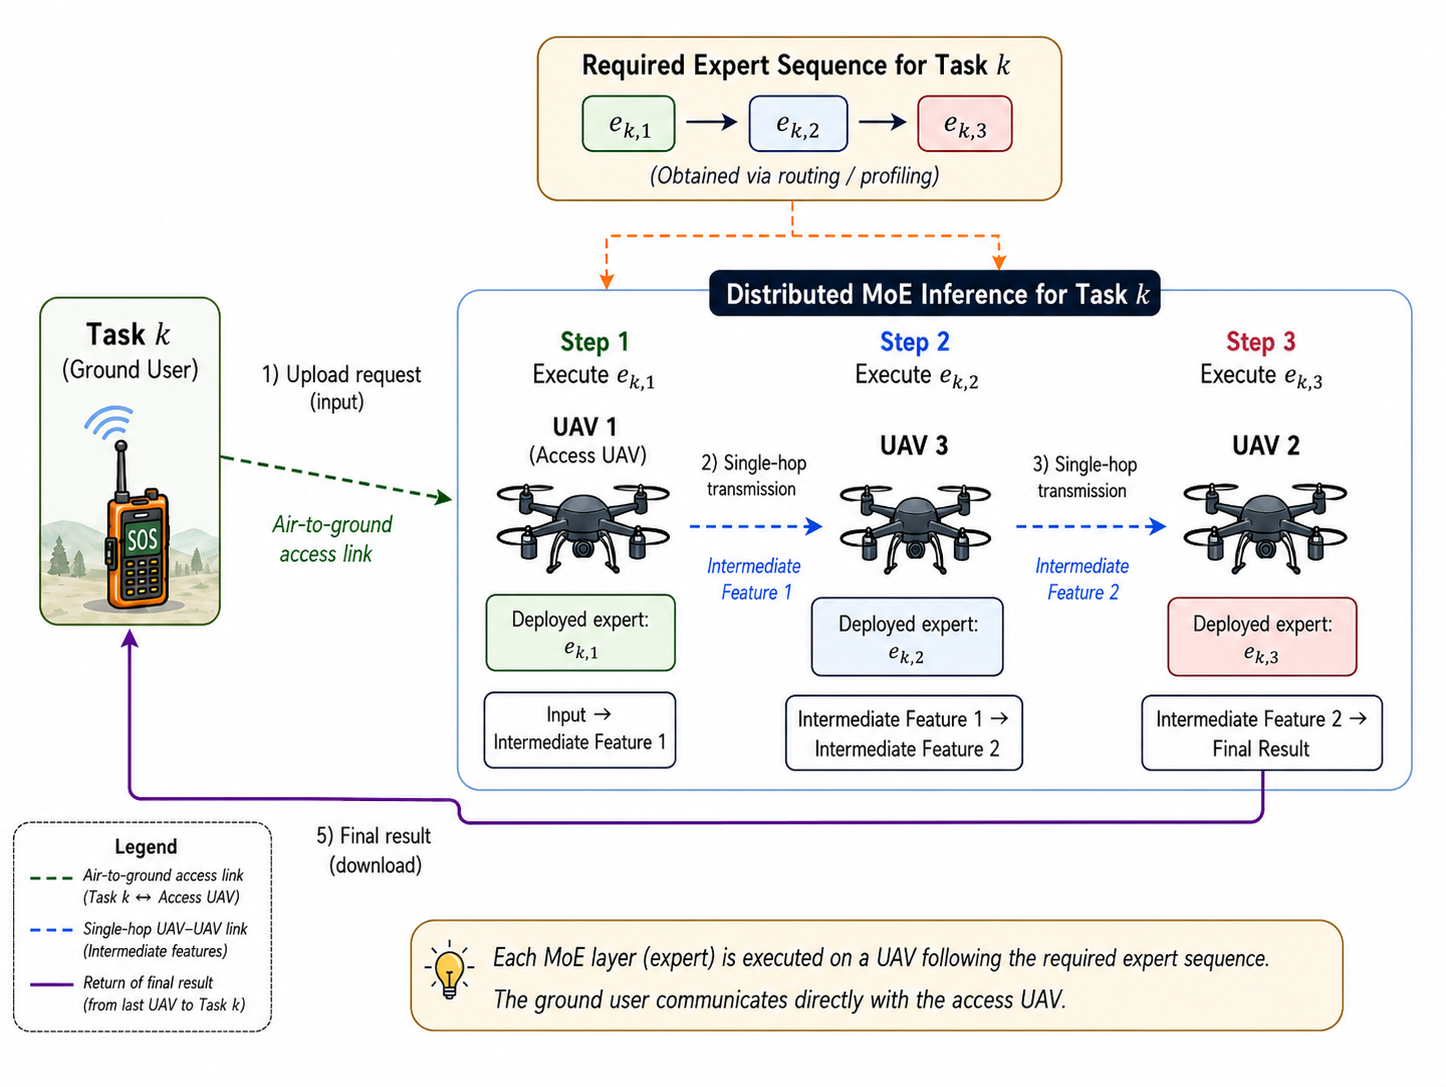
\includegraphics[width=\columnwidth,trim=0 0 0 0,clip]{system_model_uav_scenario.png}
  \caption{%准静态 UAV 边缘网络中的协同推理场景。地面任务通过空地链路接入 UAV，多个资源异构 UAV 在给定无线拓扑下协同执行 MoE 推理计算单元，并通过 UAV-UAV 链路传输中间特征，最终将推理结果返回至基站或应急指挥中心。
  Collaborative MoE inference scenario in a quasi-static UAV edge network. Ground tasks access UAVs through air-to-ground links. Heterogeneous UAVs jointly execute MoE inference units over a given wireless topology, with intermediate features transmitted via UAV-UAV links. Final results are returned to a base station or emergency command center.}
  \label{fig:system_model}
\end{figure}

\subsection{Quasi-Static UAV Network}
% 考虑一个由多个 UAV 构成的空中边缘网络，记 UAV 集合为$\mathcal{U}=\{1,2,\ldots,U\}$。每个 UAV $u\in\mathcal{U}$配备有限的计算、存储和无线通信资源，其准静态空间位置记为$\mathbf{l}_u$。在当前调度窗口内，$\mathbf{l}_u$ 作为已知参数，不作为优化变量。该假设对应灾害救援、低空巡检、应急监测等场景中UAV 在短时间内悬停或缓慢移动的情况；在该窗口内，系统主要关注当前网络拓扑下的推理资源组织，而不是 UAV 轨迹控制。
Consider a UAV edge network consisting of a set of UAVs denoted by \(\mathcal{U} = \{1, 2, \dots, U\}\). Each UAV \(u \in \mathcal{U}\) is equipped with limited computing power, memory, and wireless communication resources. The position of UAV \(u\) is denoted by \(L_u\). During each scheduling window, \(L_u\) is treated as a known parameter and is not subject to optimization. This assumption is reasonable for scenarios such as disaster response, where UAVs typically hover or move slowly. Within such a window, the system focuses on organizing inference resources based on the current network topology rather than controlling UAV trajectories.

% 每个 UAV $u$ 的可用计算能力（以 FLOP/s 计）记为 $C_u$，可用于部署推理模块或模型分片的内存容量记为 $M_u$。由于不同 UAV 的硬件平台、电池状态和后台负载可能不同，$C_u$ 和 $M_u$ 在 UAV 之间通常是异构的。这种异构性决定了不同 UAV 在协同推理中能够承担的计算量和模型状态存储量不同。
Let \(C_u\) denote the available computing power of UAV \(u\) and \(M_u\) denote its available memory capacity for storing model parameters or modules. Both \(C_u\) and \(M_u\) are heterogeneous across UAVs due to differences in hardware platforms, battery status, and background workloads.

\subsection{Wireless Model}
% UAV 网络同时包含地面节点到 UAV 的空地接入链路，以及 UAV 之间的空空协同链路。令 $\gamma_{u,v}$ 表示 UAV $u$ 到 UAV $v$ 的链路信噪比。当 $\gamma_{u,v}$ 高于给定阈值 $\gamma_{\mathrm{th}}$ 时，链路 $(u,v)$ 被认为可用。相应地，可以定义链路可用指示变量$g_{u,v}$：
% \begin{equation}
% g_{u,v} =
% \begin{cases}
% 1, & \gamma_{u,v} \ge \gamma_{\mathrm{th}},\\
% 0, & \gamma_{u,v} < \gamma_{\mathrm{th}}.
% \end{cases}
% \end{equation}
The UAV network comprises both User-UAV access links and UAV-UAV links. Let \(\gamma_{u,v}\) denote the signal-to-noise ratio (SNR) of the link from UAV \(u\) to UAV \(v\). The link is considered available if \(\gamma_{u,v}\) exceeds a predefined threshold \(\gamma_{\rm th}\). Accordingly, we define the link availability indicator as
\begin{equation}
g_{u,v} =
\begin{cases}
1, & \text{if } \gamma_{u,v} \ge \gamma_{\rm th}, \\
0, & \text{otherwise}.
\end{cases}
\end{equation}



% 若链路可用，UAV $u$ 和 UAV $v$ 之间的数据速率记为 $R_{u,v}$。该速率可以由无线带宽、发射功率、信道增益和噪声功率共同决定，也可以由在线测量得到。类似地，任务 $k$ 所在地面节点到 UAV $u$的空地接入速率记为 $R_{k,u}^{\mathrm{acc}}$。本文在协同推理执行中采用\emph{单跳 UAV-UAV 通信}：当 $g_{u,v}=1$ 时，UAV $u$ 可直接将中间特征传输到 UAV $v$；当 $g_{u,v}=0$ 时，该轮推理调度不在 $u$ 与$v$ 之间建立协同传输。
% When the link is available, the achievable data rate between UAV \(u\) and UAV \(v\) is denoted by \(R_{u,v}\).%, which depends on bandwidth, transmit power, channel gain, and noise power. 
% Similarly, let \(R_{k,u}\) denote the air-to-ground access rate from the ground node of task \(k\) to UAV \(u\).

% 采用单跳模型的原因有三点。首先，在本文考虑的准静态悬停或缓慢移动场景中，UAV 间距离和链路状态在一个调度窗口内较稳定，单跳邻域已经能够覆盖主要的低时延协同需求。其次，多跳传输需要额外决定中继 UAV、路径选择和逐跳转发时序，会把专家部署问题与网络路由问题深度耦合，显著扩大搜索空间。第三，中间特征通常规模较大，多跳转发带来的累积传输时延和中继占用可能抵消其连通性收益。基于这些考虑，本文将多跳路径选择作为可扩展方向，而在核心模型和实现中统一采用单跳可达性。
In this work, intermediate features can be transmitted directly between UAVs only if \(g_{u,v} = 1\). This design choice is motivated by three considerations. First, in quasi-static scenarios, UAV distances and channel conditions remain relatively stable within a scheduling window, making single-hop connectivity sufficient for most low-latency requirements. Second, multi-hop routing would couple the expert deployment problem with routing decisions, significantly increasing complexity. Third, intermediate features are typically large, so the cumulative delay and relay overhead of multi-hop transmission may outweigh its connectivity benefits. Consequently, multi-hop routing is left as a future extension, and we restrict all transmissions to single-hop reachable UAVs.


%\pdfcomment{这一部分属于添加的内容（没有改动原文）解释R和γ怎么来的}
% 其中，UAV \(u\) 到 UAV \(v\) 的链路信噪比 \(\gamma_{u,v}\) 可以表示为
% \begin{equation}
% \gamma_{u,v}=\frac{ P_{u} h_{u,v}}{\sigma_{u,v}^{2}},
% \end{equation}
% 其中，\( P_{u}\) 表示 UAV \(u\) 在 UAV-UAV 通信中的发射功率，\(h_{u,v}\) 表示 UAV \(u\) 到 UAV \(v\) 的信道增益，\(\sigma_{u,v}^{2}\) 表示该 UAV-UAV 链路上的噪声功率。若 \(N_0\) 表示噪声功率谱密度，\(B_{u,v}\) 表示 UAV \(u\) 到 UAV \(v\) 的通信带宽，则噪声功率可以写为
% \begin{equation}
% \sigma_{u,v}^{2}
% =
% N_0 B_{u,v}.
% \end{equation}

% 当链路 \((u,v)\) 可用时，UAV \(u\) 和 UAV \(v\) 之间的可达数据速率 \(R_{u,v}\) 可以根据 Shannon 速率模型表示为
% \begin{equation}
% R_{u,v}
% =
% B_{u,v}
% \log_2\left(1+\gamma_{u,v}\right),
% \end{equation}
% 其中，\(R_{u,v}\) 表示 UAV \(u\) 到 UAV \(v\) 的 UAV-UAV 数据速率，\(B_{u,v}\) 表示对应 UAV-UAV 链路的通信带宽，\(\gamma_{u,v}\) 表示该链路的信噪比。
The channel gains are modeled using large-scale path loss. For the air-to-ground link,
$h_{k,u} = \beta_0 d_{k,u}^{-\alpha_{\mathrm{acc}}}$,
where \(\beta_0\) is the reference channel power gain at 1 m, \(d_{k,u}\) is the distance, and \(\alpha_{\mathrm{acc}}\) is the path loss exponent. For the UAV-UAV link, $h_{u,v} = \beta_0 d_{u,v}^{-\alpha_{\mathrm{U2U}}}$, with \(d_{u,v}\) denoting the distance between UAVs \(u\) and \(v\), and \(\alpha_{\mathrm{U2U}}\) the corresponding path loss exponent. 
The SNR of the UAV-UAV link from \(u\) to \(v\) is given by
\begin{equation}\label{e2}
\gamma_{u,v} = \frac{P_u h_{u,v}}{\sigma_{u,v}^2},
\end{equation}
where \(P_u\) is the transmit power of UAV \(u\), \(h_{u,v}\) is the channel gain, and \(\sigma_{u,v}^2 = N_0 B_{u,v}\) is the noise power with \(N_0\) denoting the noise power spectral density and \(B_{u,v}\) the link bandwidth. The achievable data rate follows the Shannon capacity
\begin{equation}\label{e3}
R_{u,v} = B_{u,v} \log_2 (1 + \gamma_{u,v}).
\end{equation}

% 类似地，任务 \(k\) 所在地面节点到 UAV \(u\) 的空地接入链路信噪比记为 \(\gamma_{k,u}^{\mathrm{acc}}\)，其计算方式为
% \begin{equation}
% \gamma_{k,u}^{\mathrm{acc}}
% =
% \frac{P_{k}^{\mathrm{acc}} h_{k,u}^{\mathrm{acc}}}
% {\left(\sigma_{k,u}^{\mathrm{acc}}\right)^2},
% \end{equation}
% 其中，\(P_{k}^{\mathrm{acc}}\) 表示产生任务 \(k\) 的地面节点的接入发射功率，\(h_{k,u}^{\mathrm{acc}}\) 表示任务 \(k\) 的地面节点到 UAV \(u\) 的空地信道增益，\(\left(\sigma_{k,u}^{\mathrm{acc}}\right)^2\) 表示该空地接入链路上的噪声功率。若 \(B_{k,u}^{\mathrm{acc}}\) 表示任务 \(k\) 到 UAV \(u\) 的接入链路带宽，则有
% \begin{equation}
% \left(\sigma_{k,u}^{\mathrm{acc}}\right)^2
% =
% N_0 B_{k,u}^{\mathrm{acc}}.
% \end{equation}

% 因此，任务 \(k\) 到 UAV \(u\) 的空地接入速率 \(R_{k,u}\) 可以表示为
% \begin{equation}
% R_{k,u}
% =
% B_{k,u}^{\mathrm{acc}}
% \log_2
% \left(
% 1+\gamma_{k,u}^{\mathrm{acc}}
% \right),
% \end{equation}
% 其中，\(R_{k,u}\) 表示任务 \(k\) 的地面节点到 UAV \(u\) 的接入速率，\(B_{k,u}^{\mathrm{acc}}\) 表示对应空地接入链路的带宽，\(\gamma_{k,u}^{\mathrm{acc}}\) 表示该空地接入链路的信噪比。

% 在仿真实现中，信道增益 \(h_{u,v}\) 和 \(h_{k,u}^{\mathrm{acc}}\) 可以根据 UAV 之间或地面节点与 UAV 之间的距离、路径损耗模型、发射功率和噪声功率计算得到，也可以由在线链路测量结果给定。由上述定义可知，\(R_{u,v}\) 主要影响 UAV 之间的中间特征传输延迟，而 \(R_{k,u}\) 主要影响任务输入数据上传到 UAV 的接入延迟。

Similar to \eqref{e2} and \eqref{e3}, the SNR of the air-to-ground access link from the ground node of task \(k\) to UAV \(u\) is
$\gamma_{k,u} = \frac{P_k h_{k,u}}{\sigma_{k,u}^2}$,
with noise power $\sigma_{k,u}^2 = N_0 B_{k,u}$. The capacity is
$R_{k,u} = B_{k,u} \log_2 (1 + \gamma_{k,u})$.


% 信道增益可以由大尺度路径损耗模型得到。对于任务 \(k\) 所在地面节点到 UAV \(u\) 的空地接入链路，其信道增益表示为
% \begin{equation}
% h_{k,u}^{\mathrm{acc}}
% =
% \beta_0
% \left(d_{k,u}^{\mathrm{acc}}\right)^{-\alpha_{\mathrm{acc}}},
% \end{equation}
% 其中，\(\beta_0\) 表示参考距离 \(1\) m 处的信道功率增益，\(d_{k,u}^{\mathrm{acc}}\) 表示任务 \(k\) 所在地面节点到 UAV \(u\) 的距离，\(\alpha_{\mathrm{acc}}\) 表示空地接入链路的路径损耗指数。

% 类似地，对于 UAV \(u\) 到 UAV \(v\) 的空空链路，其信道增益可以表示为
% \begin{equation}
% h_{u,v}
% =
% \beta_0
% d_{u,v}^{-\alpha_{\mathrm{U2U}}},
% \end{equation}
% 其中，\(d_{u,v}\) 表示 UAV \(u\) 与 UAV \(v\) 之间的距离，\(\alpha_{\mathrm{U2U}}\) 表示 UAV-UAV 链路的路径损耗指数。
% } 

\subsection{Collaborative Inference Task Model}

%令 $\mathcal{K}$ 表示当前准静态调度窗口内到达的推理任务集合。每个任务 $k\in\mathcal{K}$ 由地面用户或传感器产生，输入数据大小为 $S_k^{\mathrm{in}}$，输出结果大小为 $S_k^{\mathrm{out}}$。任务首先选择一个接入 UAV上传输入数据，随后由一个或多个 UAV 协同完成模型推理，最后将推理结果返回给用户、基站或指挥中心。
Let \(\mathcal{K}\) denote the set of inference tasks arriving within the current scheduling window. Each task \(k \in \mathcal{K}\) is generated by a ground user or sensor, with input data size \(S_k^{\rm in}\) and output result size \(S_k^{\rm out}\). The task first uploads its input data to an access UAV, after which one or more UAVs collaboratively execute the inference, and the final result is returned to users.

%为了保持系统模型的通用性，本节不限定具体的模型并行策略，也不直接展开 MoE 专家的部署和执行变量。我们将待执行的推理模型抽象为若干推理计算单元，记为 $\mathcal{B}$。计算单元$b\in\mathcal{B}$ 对应一个可被部署和调度的专家权重、专家分片或层内计算块，具有执行该单元所需的计算量 $F_b$ 和存放其参数所需的内存占用 $W_b$。对每个任务 $k$，其当前推理路径所需的计算单元构成一个有序子集 $\mathcal{B}_k\subseteq\mathcal{B}$，按线性执行顺序排列。在后续 AeroMoE 设计中，这些抽象计算单元将被进一步具体化为 MoE 模型中的逐层 expert FFN。
To maintain generality, we abstract the inference model as a set of computation units \(\mathcal{B}\). Each unit \(b \in \mathcal{B}\) represents a deployable module (e.g., an expert weight, a shard, or a layer block) with computation requirement \(F_b\) and memory footprint \(W_b\). For task \(k\), the required computation units form an ordered subset \(\mathcal{B}_k \subseteq \mathcal{B}\).
% {\color{red}
% 按线性执行顺序排列，并记 $L_k=|\mathcal{B}_k|$ 为任务 $k$ 的
% 推理步骤数。在后续 AeroMoE 设计中，这些抽象
% 计算单元将被进一步具体化为 MoE 模型中的逐层 expert FFN。\pdfcomment{这一部分属于添加的内容（没有改动原文）用于后边修改pkuv改成了，pkluv,多了l表示任务执行的第几层。}
% } 
The computation units required by task \(k\) form an ordered subset \(\mathcal{B}_k \subseteq \mathcal{B}\) arranged according to their linear execution order, where \(L_k = |\mathcal{B}_k|\) denotes the number of inference steps. In the AeroMoE design, these abstract computation units are instantiated as the layer-wise expert feed-forward network (FFN) modules of the MoE model.


%系统需要决定任务 $k$ 的接入 UAV、参与协同的 UAV 集合、各推理模块在 UAV 上的执行分配，以及不同 UAV 之间的中间特征传输路径。令 $y_{k,u}\in\{0,1\}$ 表示任务 $k$ 是否由 UAV $u$ 接入；令$s_{k,b,u}\in\{0,1\}$ 表示任务 $k$ 的推理模块 $b$ 是否在 UAV $u$上执行；令 $p_{k,u,v}\in\{0,1\}$ 表示任务 $k$ 是否需要在 UAV $u$和 UAV $v$ 之间传输中间特征。这里的 $s_{k,b,u}$ 和 $p_{k,u,v}$是通用协同推理层面的抽象决策变量，后续可以根据具体 MoE 路由和专家部署方式进一步实例化。
The system determines the access UAV for each task, the set of participating UAVs, the assignment of computation units to UAVs, and the transmission paths for intermediate features. We introduce the following binary decision variables, \(y_{k,u} \in \{0,1\}\) indicates whether task \(k\) accesses UAV \(u\) and
\(s_{k,b,u} \in \{0,1\}\) indicates whether computation unit \(b\) of task \(k\) is executed on UAV \(u\). 
%\(p_{k,u,v} \in \{0,1\}\) indicates whether intermediate features must be transmitted from UAV \(u\) to UAV \(v\) for task \(k\).
%These variables are defined at the level of general collaborative inference and will be instantiated for MoE models in subsequent sections.
% {\color{red}
% 令 $p_{k,l,u,v}\in\{0,1\}$ 表示任务 $k$ 在第 $l$ 个相邻
% 推理步骤之间是否需要从 UAV $u$ 向 UAV $v$ 传输中间特征。这里的
% $s_{k,b,u}$ 和 $p_{k,l,u,v}$
% 是通用协同推理层面的抽象决策变量，后续可以根据具体 MoE 路由和
% 专家部署方式进一步实例化。\pdfcomment{这一部分属于改动原文的部分（还没有改原文）：这里吧原来的pkuv改成了，pkluv,多了l表示任务执行的第几层。}
% } 
We introduce the binary variable \( p_{k,l,u,v} \in \{0,1\} \) to indicate whether intermediate features must be transmitted from \( u \) to \( v \) between the \( l \)-th and \( (l+1) \)-th execution steps of task \( k \). Both \( s_{k,b,u} \) and \( p_{k,l,u,v} \) are abstract decision variables defined for general collaborative inference.%; they will be instantiated based on the specific MoE routing and expert deployment decisions in later sections.


\subsection{End-to-End Delay Model}

% 任务 $k$ 的端到端推理延迟由接入延迟、协同计算延迟、UAV-UAV中间特征传输延迟和结果回传延迟组成：
% \begin{equation}
% D_k = D_k^{\mathrm{acc}} + D_k^{\mathrm{compute}}
%     + D_k^{\mathrm{trans}} + D_k^{\mathrm{return}} .
% \end{equation}
The end-to-end latency of task \(k\) consists of four components, i.e., uplink delay, computation delay, transmission delay, and downlink delay, 
\begin{equation}
D_k = D_k^{\rm ul} + D_k^{\rm comp} + D_k^{\rm trans} + D_k^{\rm dl}.
\end{equation}
They are given as %\pdfcomment{我又看了一下，我感觉好像没有问题，因为这里的yku表示任务k通过哪一个无人机u接入，只有一个无人机接入任务k，当k确定的时候，是可以通过yku找到对应无人机的}
\begin{equation}
D_k^{\rm ul} = \sum_{u \in \mathcal{U}} y_{k,u} \frac{S_k^{\rm in}}{R_{k,u}},
\end{equation}
\begin{equation}
D_k^{\rm comp} = \sum_{b \in \mathcal{B}} \sum_{u \in \mathcal{U}} s_{k,b,u} \frac{F_b}{C_u},
\end{equation}
%\begin{equation}
%D_k^{\rm trans} = \sum_{u \in \mathcal{U}} \sum_{v \in \mathcal{U}, v \ne u} p_{k,u,v} \frac{S_{k,u,v}^{\rm mid}}{R_{u,v}},
%\end{equation}
{\color{black}
\begin{equation}
D_k^{\mathrm{trans}}
= \sum_{l=1}^{L_k-1}
  \sum_{u\in\mathcal{U}}\sum_{v\in\mathcal{U},v\ne u}
   p_{k,l,u,v}\frac{S_{k,l}^{\mathrm{mid}}}{R_{u,v}} ,
\end{equation}%\pdfcomment{这一部分属于改动原文的部分（还没有改原文）：因为前边的p修改了，所以这里也改了一下，我看这样好像多一个l会更规范一些。但是这个l和前边定义uav的位置L好像重复了}
%其中 $p_{k,l,u,v}=1$ 仅在 $g_{u,v}=1$ 时允许取值为 $1$；若两个 UAV不能直接通信，则该任务步骤不能直接在二者之间迁移中间特征，而需在调度时选择其他单跳可达的执行 UAV。
where \( p_{k,l,u,v} \) can take the value 1 only if \( g_{u,v} = 1 \). If UAVs \( u \) and \( v \) are not directly connected, the intermediate features cannot be transmitted between them. In this case, the scheduler must select another reachable UAV for execution. 
} 

%\pdfcomment{q1：是否需要定义一下u*k,l.--已经定义q2：感觉需要加一个最后的无人机能和k通信的约束。}
% \begin{equation}
% D_k^{\rm dl} = \frac{S_k^{\rm out}}{R_k^{\rm return}},
% \end{equation}
{\color{black}
\begin{equation}
D_k^{\rm dl}
=
\frac{S_k^{\mathrm{out}}}{R_{u^*_{k,L_k},k}},
\end{equation}
%其中 \(R_{u^*_{k,L_k},k}\) 表示任务 \(k\) 最后一步专家所在 UAV 到任务目的节点的有效下行回传速率，$u^*_{k,l}$ 表示任务 $k$ 的第 $l$ 步专家实际选择的执行 UAV，因此 $u^*_{k,L_k}$ 即为任务 $k$ 最后一步专家所在的 UAV。
where \(L_k\) is the number of execution steps and \( u_{k,l}^* \) denotes the UAV chosen to execute the \( l \)-th step of task \( k \), so \( u_{k,L_k}^* \) is the UAV selected for the final step. The term \( R_{u_{k,L_k}^*,k} \) represents the effective downlink rate from this UAV to the destination of task \( k \).
}

% 接入延迟表示输入数据从地面节点上传到接入 UAV 的时间：
% \begin{equation}
% D_k^{\mathrm{acc}}
% = \sum_{u\in\mathcal{U}} y_{k,u}
%   \frac{S_k^{\mathrm{in}}}{R_{k,u}^{\mathrm{acc}}} .
% \end{equation}

% 协同计算延迟由各推理模块在被分配 UAV 上的执行时间决定：
% \begin{equation}
% D_k^{\mathrm{compute}}
% = \sum_{b\in\mathcal{B}}\sum_{u\in\mathcal{U}}
%    s_{k,b,u}\frac{F_b}{C_u}.
% \end{equation}

% UAV-UAV 传输延迟由中间特征大小和协同链路速率决定。令
% $S_{k,u,v}^{\mathrm{mid}}$ 表示任务 $k$ 在 UAV $u$ 和 UAV $v$
% 之间需要传输的中间特征大小，则
% \begin{equation}
% D_k^{\mathrm{trans}}
% = \sum_{u\in\mathcal{U}}\sum_{v\in\mathcal{U},v\ne u}
%    p_{k,u,v}\frac{S_{k,u,v}^{\mathrm{mid}}}{R_{u,v}} .
% \end{equation}
% 其中 $p_{k,u,v}=1$ 仅在 $g_{u,v}=1$ 时允许取值为 $1$；若两个 UAV不能直接通信，则该任务步骤不能直接在二者之间迁移中间特征，而需在调度时选择其他单跳可达的执行 UAV。

% 结果回传延迟将推理输出从最终执行 UAV 传输至用户、基站或指挥中心：
% \begin{equation}
% D_k^{\mathrm{return}}
% = \frac{S_k^{\mathrm{out}}}{R_k^{\mathrm{return}}},
% \end{equation}
% 其中 $R_k^{\mathrm{return}}$ 为最终执行 UAV 到目的节点的等效回传速率。由于推理输出通常远小于输入数据和中间特征，$D_k^{\mathrm{return}}$可以作为较小的常数项处理。

\subsection{Optimization Problem}

Given UAV positions, link states, computation and memory resources, and the set of tasks, the objective is to minimize the expected end-to-end latency, which is 
% \begin{equation}\label{e16}
% \min_{y,s,p} \ \mathbb{E}\left[ \sum_{k \in \mathcal{K}} D_k \right],
% \end{equation}
% subject to the following constraints.
%\pdfcomment{相比原来只有D_k多加了omega_k。这时候和第四章总任务一致}

\begin{equation}\label{e16}
\min_{y,s,p} \ \mathbb{E}\left[D_{\mathrm{total}} \right],
\end{equation}
%where $D_{\mathrm{total}} = \sum_{k\in\mathcal{K}} \omega_k D_k$. \(\omega_k\)表示任务k的权重，反应任务优先级。
where \( D_{\mathrm{total}} = \sum_{k \in \mathcal{K}} \omega_k D_k \) and \(\omega_k > 0\) is the priority weight of task \(k\). Each task accesses exactly one UAV, i.e., 
\begin{equation}
\text{C1: } \sum_{u \in \mathcal{U}} y_{k,u} = 1, \quad \forall k \in \mathcal{K}.
\end{equation}
Each computation unit must be assigned to exactly one UAV for execution, i.e.,
\begin{equation}
\text{C2: } \sum_{u \in \mathcal{U}} s_{k,b,u} = 1, \quad \forall k \in \mathcal{K}, \, b \in \mathcal{B}.
\end{equation}
The total computation load on each UAV cannot exceed its available budget, i.e.,
\begin{equation}
\text{C3: } \sum_{k \in \mathcal{K}} \sum_{b \in \mathcal{B}} s_{k,b,u} F_b \le C_u^{\max}, \quad \forall u \in \mathcal{U}.
\end{equation}
%\pdfcomment{这一部分属于改动原文的部分（还没有改原文）：C3这个约束，我当时发现代码没有考虑这点，所以删掉了-------------------如果删了的话，要做一个UAV消耗的平均F。。。。想一下咋改动这个}
The memory usage on each UAV cannot exceed its capacity, i.e.,
\begin{equation}
\text{C4: } \sum_{b \in \mathcal{B}} m_{b,u} W_b \le M_u, \quad \forall u \in \mathcal{U},
\end{equation}
and execution is permitted only on UAVs where the module is deployed, i.e.,
\begin{equation}
\text{C5: } s_{k,b,u} \le m_{b,u}, \quad \forall k \in \mathcal{K}, \, b \in \mathcal{B}, \, u \in \mathcal{U}.
\end{equation}
Intermediate feature transmission is restricted to single-hop links, i.e., 
%\begin{equation}
%\text{C6: } p_{k,u,v} = 1 \implies g_{u,v} = 1, \quad \forall k \in \mathcal{K}, \, u,v \in \mathcal{U}.
%\end{equation}
%
%Finally, for each task \(k\) with linear execution order \(b_{k,1} \prec b_{k,2} \prec \cdots \prec b_{k,L_k}\), transmission is required between adjacent modules executed on different UAVs:
%\begin{equation}
%\text{C7: } s_{k,b_{k,l},u} = 1 \land s_{k,b_{k,l+1},v} = 1 \land u \ne v \implies p_{k,u,v} = 1,
%\end{equation}
%for all \(l = 1, \dots, L_k-1\).

%\pdfcomment{这一部分属于改动原文的部分（还没有改原文）因为p的改动，所以C6和C7也要改一下}
\begin{multline}
\text{C6: } p_{k,l,u,v}=1 \Rightarrow g_{u,v}=1,\\
\forall k\in\mathcal{K},\; l=1,\ldots,L_k-1,\; u,v\in\mathcal{U}.
\end{multline}
% $b_{k,1} \prec_k b_{k,2} \prec_k \cdots \prec_k b_{k,L_k}$，
% 其中 $b_{k,l}\in\mathcal{B}$、$L_k=|\mathcal{B}_k|$ 为任务 $k$ 所需
% 执行的模块总数。若两个相邻模块被分配到不同的 UAV 上执行，
% 则必须在这两个 UAV 之间传输中间特征：
For each task \(k\) with linear execution order \(b_{k,1} \prec_k b_{k,2} \prec_k \cdots \prec_k b_{k,L_k}\), where \(b_{k,l} \in \mathcal{B}\) and \(L_k = |\mathcal{B}_k|\), if two consecutive modules are assigned to different UAVs, intermediate features must be transmitted between them,
\begin{multline}
\text{C7: } s_{k,b_{k,l},u}\!=\!1 \;\land\; s_{k,b_{k,l+1},v}\!=\!1
\;\land\; u\neq v \;\Longrightarrow\; p_{k,l,u,v}\!=\!1,\\[2pt]
\forall\,k\in\mathcal{K},\; l\!=\!1,\ldots,L_k-1,\; u,v\in\mathcal{U}.
\label{eq:p_s_coupling}
\end{multline}


This formulation captures the essential characteristics of collaborative inference in quasi-static UAV edge networks, where task access, computation assignment, and feature transmission must be jointly optimized under resource and connectivity constraints. Subsequent sections will instantiate this general model for MoE inference by specializing the computation units to experts and incorporating similarity-aware deployment and scheduling.

% 在给定 UAV 位置、链路状态、计算资源、内存资源和任务集合的条件下，系统目标是在满足资源和连通性约束的同时，最小化任务的期望端到端推理延迟：
% \begin{equation}
% \min_{\mathbf{y},\mathbf{s},\mathbf{p}}
% \quad
% \mathbb{E}\left[\sum_{k\in\mathcal{K}} D_k\right].
% \end{equation}

% 上述目标受到以下约束。首先，每个任务只能选择一个接入 UAV：
% \begin{equation}
% \sum_{u\in\mathcal{U}} y_{k,u}=1,\quad \forall k\in\mathcal{K}.
% \end{equation}

% 其次，每个推理模块必须被分配到能够参与协同推理的 UAV 上执行：
% \begin{equation}
% \sum_{u\in\mathcal{U}} s_{k,b,u}=1,\quad
% \forall k\in\mathcal{K}, b\in\mathcal{B}.
% \end{equation}

% 第三，UAV 的计算负载不能超过其在当前调度窗口内的可用计算预算。令 $C_u^{\max}$ 表示 UAV $u$ 在当前调度窗口内的最大可用计算量（以 FLOPs 计），则有
% \begin{equation}
% \sum_{k\in\mathcal{K}}\sum_{b\in\mathcal{B}}
% s_{k,b,u}F_b \le C_u^{\max},\quad \forall u\in\mathcal{U}.
% \end{equation}

% 第四，部署在每个 UAV 上的模型模块或模型分片不能超过其内存容量。令 $m_{b,u}\in\{0,1\}$ 表示推理模块 $b$ 是否被部署在 UAV $u$ 上，则有
% \begin{equation}
% \sum_{b\in\mathcal{B}} m_{b,u}W_b \le M_u,\quad
% \forall u\in\mathcal{U},
% \end{equation}
% 并且模块只能在已部署该模块的 UAV 上执行：
% \begin{equation}
% s_{k,b,u}\le m_{b,u},\quad
% \forall k\in\mathcal{K}, b\in\mathcal{B}, u\in\mathcal{U}.
% \end{equation}

% 第五，任务的中间特征传输必须满足 UAV-UAV 连通性要求：
% \begin{equation}
% p_{k,u,v}=1 \Rightarrow g_{u,v}=1,\quad
% \forall k\in\mathcal{K}, u,v\in\mathcal{U}.
% \end{equation}
% 该约束表示本文只允许中间特征在单跳可达的 UAV 对之间传输。

% 第六，中间特征传输与模块执行分配之间的耦合关系需要显式刻画。对于每个任务 $k$，记其推理模块的线性执行顺序为
% $b_{k,1} \prec_k b_{k,2} \prec_k \cdots \prec_k b_{k,L_k}$，
% 其中 $b_{k,l}\in\mathcal{B}$、$L_k=|\mathcal{B}_k|$ 为任务 $k$ 所需执行的模块总数。若两个相邻模块被分配到不同的 UAV 上执行，则必须在这两个 UAV 之间传输中间特征：
% \begin{multline}
% s_{k,b_{k,l},u}=1 \;\land\; s_{k,b_{k,l+1},v}=1
% \;\land\; u\neq v \;\Longrightarrow\; p_{k,u,v}=1,\\[2pt]
% \forall\,k\in\mathcal{K},\; l=1,\ldots,L_k-1,\; u,v\in\mathcal{U}.
% \label{eq:p_s_coupling}
% \end{multline}
% 在后续 Design 章节中，该执行顺序被具体化为 MoE 模型的逐层专家执行序列（第~\ref{sec:inference_scheduling}~节中 $\mathcal{C}_{k,l}$的定义即依赖于这一相邻步的传输逻辑）。

% 该通用问题刻画了准静态 UAV 边缘网络中的协同推理本质：在无线链路受限、资源异构且内存受限的空中边缘节点之间，联合决定任务接入、协同执行和中间特征传输，以降低端到端推理延迟。后续章节将在该通用模型基础上，将抽象的推理模块部署和执行分配进一步具体化为MoE 专家候选构造、相似性感知专家部署和逐层单跳推理调度问题。



% ==============================================================
\section{Proposed Design}
\label{sec:design}
% ==============================================================


%在协同推理优化问题\eqref{e16}中，系统需要联合优化专家部署变量 $m_{e,u}$、任务接入变量 $y_{k,u}$、专家执行变量 $s_{k,l,u}$ 以及中间特征传输选择变量 {\color{red}$p_{k,l,u,v}$} 。\pdfcomment{这里p的符号变了，多了l}该联合优化问题的搜索空间随 UAV 数量、专家数量和任务数量呈指数增长，在实时性要求下难以直接求解。
In the optimization problem~\eqref{e16}, the system must simultaneously optimize the expert deployment variables \(m_{e,u}\), task access variables \(y_{k,u}\), expert execution variables \(s_{k,l,u}\), and intermediate feature transmission variables \(p_{k,l,u,v}\). The search space of this problem grows exponentially with the number of UAVs, experts, and tasks, rendering direct solution intractable under real-time constraints.

%为此，AeroMoE 将联合优化问题解耦为任务需求匹配、相似候选专家构造、通信感知动态部署与推理调度四个顺序阶段，每个阶段仅需处理一个规模可控的子问题。各阶段之间单向递进，前一阶段的输出作为后一阶段的输入，避免了迭代式联合优化带来的复杂交替求解过程。AeroMoE 牺牲了交替优化的全局迭代搜索能力，换取了准静态 UAV 调度窗口下更适合实时执行的低复杂度部署策略.
To address this challenge, AeroMoE decouples the joint optimization into five sequential stages as illustrated in Fig.~\ref{fig:design_flow}. Each stage solves a smaller, tractable subproblem, and the stages are executed in a feed-forward manner, with the output of one stage serving as the input to the next. This design trades the global search capability of iterative alternating optimization for significantly lower computational complexity, which is essential for real-time operation within quasi-static UAV scheduling windows. The five stages are defined as follows.

%{\color{red}AeroMoE 牺牲了交替优化的全局迭代搜索能力，换取了准静态 UAV 调度窗口下更适合实时执行的低复杂度部署策略.} 
%\pdfcomment{这个光说靠【各阶段之间单向递进】也避免不了，AO框架在某一次迭代中，就是各阶段之间单向递进的。之所以多次为了收敛到最优：：：：方案1：（只进行解释）需要强调的是，AeroMoE 并不试图通过多轮交替优化来逼近联合优化问题的局部最优解。相反，本文将任务需求分布、专家相似替代关系、单跳链路可达性、链路速率、UAV 计算能力、网络位置以及专家内存代价等关键耦合因素提前编码到部署评分函数中，使专家部署阶段能够在不反复调用在线调度过程的情况下，对后续推理执行中的主要延迟来源进行近似感知。同时，动态贪心部署中的冗余惩罚会随着已部署专家集合实时更新，从而以较低复杂度模拟部署决策之间的边际收益变化。换言之，AeroMoE 牺牲了交替优化的全局迭代搜索能力，换取了准静态 UAV 调度窗口下更适合实时执行的低复杂度部署策略；其有效性将在实验部分通过与多种基线方法的端到端延迟对比进行验证。-----方案2：加“小规模近似最优/迭代改进实验”，不加完整 AO。。对比性能差距，如果差距小的话，就用实验结果说明该方法复杂度低了，并且性能没有差太多}


\begin{figure}[!t]
  \centering
  \includegraphics[width=\columnwidth,trim= 30 200 30 100,clip]{design_flow.pdf}
  \caption{AeroMoE decouples the joint optimization into five sequential stages, i.e., task demand matching, similarity-aware candidate construction, communication-aware dynamic deployment, and inference scheduling.}
  \label{fig:design_flow}
\end{figure}
%\pdfcomment{下边我看改成5个步骤了，那么是不是这个1备注要改5个，2引用这个图的部分也要改}

%图~\ref{fig:design_flow} 展示了 AeroMoE 设计阶段的整体流程,分为以下四个部分.
%\subsubsection{任务需求匹配} 将地面任务按最小接入延迟归属到各 UAV 区域.统计每个 UAV 区域的直接专家需求分布 $\mathrm{Demand}(r,u)$。
\subsubsection{Task Demand Matching} Ground tasks are assigned to UAV regions according to minimum access delay. The direct expert demand distribution \(\mathrm{Demand}(r,u)\) is then computed for each UAV region.
%设计并基于专家权重相似度 $\mathrm{Sim}(r,e)$，为每个原始需求专家 $r$ 构造可替代专家集合 $\mathcal{A}(r)$，将原始专家需求扩展为候选专家的有效需求 $\mathrm{Demand}^{\mathrm{eff}}(e,u)$。
\subsubsection{Similarity-Aware Candidate Construction} For each originally required expert \(r\), a substitutable expert set \(\mathcal{A}(r)\) is constructed based on expert weight similarity \(\mathrm{Sim}(r,e)\). The original demands are then extended to effective demands \(\mathrm{Demand}^{\mathrm{eff}}(e,u)\) over the candidate experts.
\subsubsection{Communication-Aware Expert Placement Scoring} For each candidate deployment pair \((e,u)\), a base deployment score \(\mathrm{BaseScore}(e,u)\) is computed by jointly considering link availability \(g_{v,u}\), UAV computing power \(C_u\), and network topology. 
%综合考虑通信可达性 $g_{v,u}$、计算能力 $C_u$ 和网络拓扑位置，为每个候选部署对 $(e,u)$ 计算基础部署得分 $\mathrm{BaseScore}(e,u)$。在 UAV 内存约束下通过动态贪心算法生成最终专家部署方案$\{m_{e,u}\}$.
\subsubsection{Dynamic Expert Placement} A dynamic greedy algorithm then generates the final deployment decisions \(\{m_{e,u}\}\) under per-UAV memory constraints.

\subsubsection{Inference Scheduling} A per-layer greedy scheduler is designed to determine the end-to-end task latency \(D_{\mathrm{total}}\).
%设计逐层贪心推理调度策略计算端到端任务延迟$D_{\mathrm{total}}$。

%本章中, System Model 中的抽象推理模块 $b\in\mathcal{B}$ 在 Design 阶段被实例化为具体的 MoE 专家 $e\in\mathcal{E}_{\mathrm{cand}}$，模块执行顺序$\prec_k$ 被具体化为 MoE 模型的逐层专家执行序列.第 $l$ 步原始所需专家记为 $e_{k,l}$。抽象执行分配变量 $s_{k,b,u}$ 被细化为逐步专家执行指示变量 $s_{k,l,u}$, i.e.,
In this design phase, the abstract computation units \(b \in \mathcal{B}\) from the System Model are instantiated as concrete MoE experts \(e \in \mathcal{E}_{\mathrm{cand}}\). The linear execution order \(\prec_k\) is specialized to the layer-wise expert FFN sequence of the MoE model, where the expert required at step \(l\) is denoted by \(e_{k,l}\). Accordingly, the abstract execution variables \(s_{k,b,u}\) are refined to per-step execution indicators \(s_{k,l,u}\), defined as
% \begin{multline}
% s_{k,l,u}=1 \;\Longleftrightarrow\; \text{任务 }k\text{ 的第 }l\text{ 步专家在 UAV }u
% \text{ 上执行},\\[2pt]
% \forall\,k\in\mathcal{K},\; l=1,\ldots,L_k,\; u\in\mathcal{U}.
% \label{eq:sklu_def}
% \end{multline}
% 传输选择变量 $p_{k,u,v}$ 在 Design 阶段不再显式作为决策变量，而是由推理调度中逐步的当前 UAV $cur$ 到目标 UAV $u$ 的单跳传输隐式确定.%（对应式~(\ref{eq:candidate_exec}) 中 $u=cur$ 或 $g_{cur,u}=1$ 的条件；多跳传输简化为单跳的理由见第~\ref{sec:demand_modeling}~节）。
\begin{equation}
s_{k,l,u} = 1 \;\Longleftrightarrow\; \text{the $l$-th expert of $k$ is executed on $u$},
\end{equation}
for all \(k \in \mathcal{K}\), \(l = 1, \dots, L_k\), and \(u \in \mathcal{U}\).
The transmission variables \(p_{k,l,u,v}\) are no longer treated as explicit decision variables during deployment. Instead, they are implicitly determined during inference scheduling by the single-hop transmission from the current UAV \(cur\) to the target UAV \(u\).
% ==============================================================
% \subsection{Task Demand Matching}
% \label{sec:demand_modeling}

% 本节依次定义任务默认接入归属、直接专家需求统计。
% \subsubsection{任务默认接入的归属 UAV}
% 对于每个任务 $k\in\mathcal{K}$，AeroMoE 根据最小接入延迟原则将其归属到默认接入 UAV
% \begin{equation}
% u_k^a = \arg\min_{u\in\mathcal{U}} \frac{S_k^{\mathrm{in}}}{R_{k,u}},
% \label{eq:default_access}
% \end{equation}
% 其中 $S_k^{\mathrm{in}}$ 为任务 $k$ 的输入数据大小，$R_{k,u}$ 为任务 $k$ 到 UAV $u$ 的空地接入速率。{\color{red}通过对每个任务遍历所有UAV，选入接入延迟最小的UAV，因此每个任务最终只有一个默认接入UAV，从而实现了约束C1.} 归属完成后，任务 $k$ 的专家需求将全部统计到其默认接入 UAV$u_k^a$ 所在区域，用于下一步的需求分布统计。

% \subsubsection{直接专家需求}
% 在任务接入归属确定后，UAV $u$ 区域对原始专家 $r$ 的直接需求函数定义为：
% \begin{equation}
% \mathrm{Demand}(r,u) = \sum_{k:\,u_k^a = u} \omega_k \, q_{k,r},
% \label{eq:demand}
% \end{equation}
% 其中 $\omega_k$ 为任务 $k$ 的权重（反映任务优先级或历史到达频率），$q_{k,r}$ 为任务 $k$ 对专家 $r$ 的需求强度。若 MoE 模型提供 gatingnetwork 输出的路由权重，则 $q_{k,r}$ 可取任务 $k$ 所有输入 token 对专家 $r$ 的 gating score 之和；若无 gating 先验信息，则按专家 $r$在任务 $k$ 所需专家序列中的出现次数统计。$\mathrm{Demand}(r,u)$ 仅描述任务\emph{原本需要}哪些原始专家，相似专家替代和有效需求扩展尚未在此处处理，

% % \subsubsection{UAV-UAV 通信}
% % %System Model（第~\ref{sec:system}~节）中允许中间特征通过多跳 UAV-UAV路径传输。然而，在专家部署规划阶段，若考虑全路径多跳传输，部署评分将与具体的端到端路径选择深度耦合，显著增加问题复杂度。此外，在准静态UAV 悬停场景和典型任务需求密度下，单跳通信已能覆盖 UAV 之间的主要协同需求，多跳传输带来的额外延迟累积往往抵消其连通性扩展收益。因此，AeroMoE 在 Design 阶段将 UAV-UAV 协同通信\emph{简化为单跳可达模型}。最终推理调度中的真实端到端传输延迟仍按 System Model 中的定义，根据实际所选路径的等效传输时延计算。

% % UAV $v$ 到 UAV $u$ 的单跳可达指示变量定义为一个二元变量,
% % \begin{equation}
% % g_{v,u} =
% % \begin{cases}
% % 1, & \text{UAV } v \text{ 可单跳访问 UAV } u,\\
% % 0, & \text{否则}.
% % \end{cases}
% % \label{eq:single_hop_g}
% % \end{equation}

% %对应的单跳数据传输速率为 $R_{v,u}$。令 $R_{\max} = \max_{v,u\in\mathcal{U},\,v\neq u} R_{v,u}$ 为所有可用UAV-UAV 单跳链路中的最大速率，用于后续部署评分中的速率归一化。这些链路信息将直接被第~\ref{sec:placement_scoring}~节的通信感知部署评分和第~\ref{sec:greedy_scheduling}~节的推理调度所使用。

% % ==============================================================
% \subsection{Similarity-Aware Candidate Expert Construction}
% \label{sec:similarity_candidate}

% %本节是 AeroMoE 方法的关键创新之一，解决的问题是：\emph{部署候选专家从哪里来？是否只考虑任务原本需要的专家？相似专家如何加入候选集合？替代专家的有效需求如何计算？}
% 本节依次定义原始所需专家集合、可替代专家集合、候选专家集合和有效需求四个概念。

% \subsubsection{任务原本需要的原始专家集合}

% % 令 $E_k$ 表示任务 $k$ 的专家执行序列,由 MoE gating network 的路
% % 由决策或任务预配置确定。所有任务原本需要的原始专家集合为：
% % \begin{equation}
% % \mathcal{E}_{\mathrm{req}} = \{\,r \mid \exists k\in\mathcal{K},\;
% % r \in E_k\,\}.
% % \label{eq:ereq}
% % \end{equation}
% % %例如，若任务 $k_1$ 需要专家序列 $\{E_1, E_2\}$，任务 $k_2$ 需要$\{E_2, E_3\}$，则 $\mathcal{E}_{\mathrm{req}} = \{E_1, E_2, E_3\}$。
% % $\mathcal{E}_{\mathrm{req}}$ 是所有后续候选构造的起点。
% \pdfcomment{这个符号的构造有点问题吧.Ek是任务k的顺序,k=1,2,3,4,5有E1,E2,3,4,5,那怎么例如，若任务 k_1 需要专家序列 {E_1, E_2}，}

% {\color{red}
% 令任务 $k$ 的原始专家执行序列为$\mathbf{e}_k=(e_{k,1},e_{k,2},\ldots,e_{k,L_k})$，该序列由 MoEgating network 的路由决策或任务预配置确定。其中 $L_k$ 表示任务 $k$的专家执行步数，$e_{k,l}$ 表示任务 $k$ 在第 $l$ 个 MoE 层或第 $l$个执行位置所需的原始专家。所有任务原本需要的原始专家集合为：
% \begin{equation}
% \mathcal{E}_{\mathrm{req}}
% = \{\,r \mid \exists k\in\mathcal{K},\;
% \exists l\in\{1,\ldots,L_k\},\; r=e_{k,l}\,\}.
% \label{eq:ereq}
% \end{equation}
% %例如，若任务 $k_1$ 的专家执行序列为 $(E_1,E_2)$，任务 $k_2$ 的专家执行序列为 $(E_2,E_3)$，则$\mathcal{E}_{\mathrm{req}} = \{E_1, E_2, E_3\}$。$\mathcal{E}_{\mathrm{req}}$ 是所有后续候选构造的起点。
% } 



% \subsubsection{可替代专家集合}

% 对于任意原始专家 $r\in\mathcal{E}_{\mathrm{req}}$，其可替代专家集合
% 包含 $r$ 本身以及所有与 $r$ 足够相似的专家：
% % \begin{equation}
% % \mathcal{A}(r) = \{r\} \cup \{\,e \mid \mathrm{Sim}(r,e) \ge \xi\,\},
% % \label{eq:ar}
% % \end{equation}
% \pdfcomment{注释：把定义改了一下，之前可能会定义不相关的e：？？？？一个别的疑惑，到底是改用e（e只定义了ek），还是E（上边没有定义，用的话需要定义吧），，，chatgpt说还是用e，E表示具体专家，e是专家变量，ek是任务k用的专家序列，ek，l是专家k用到的第l个专家/所以说不矛盾}
% \begin{equation}
% \mathcal{A}(r) = \{r\} \cup \{\,e\in\mathcal{E} \mid \mathrm{Sim}(r,e) \ge \xi\,\},
% \label{eq:ar}
% \end{equation}
% 其中 $\mathrm{Sim}(r,e)\in[0,1]$ 为专家 $r$ 与专家 $e$ 的相似度，
% $\xi\in[0,1]$ 为相似度阈值。本文采用专家 FFN 权重矩阵展平后的余弦相似度作为 $\mathrm{Sim}(r,e)$：
% \begin{equation}
% \mathrm{Sim}(r,e) =
% \frac{1}{2}\left(
% 1+
% \frac{\bigl\langle \mathrm{vec}(\mathbf{W}_r),\,
%                 \mathrm{vec}(\mathbf{W}_e) \bigr\rangle}
%      {\|\mathrm{vec}(\mathbf{W}_r)\|_2\,
%       \|\mathrm{vec}(\mathbf{W}_e)\|_2}
% \right),
% \label{eq:sim}
% \end{equation}
% 其中 $\mathbf{W}_r$、$\mathbf{W}_e$ 分别为专家 $r$ 和专家 $e$ 的 FFN权重参数,将多层全连接权重矩阵展平后拼接为单一向量，$\mathrm{vec}(\cdot)$ 为矩阵向量化操作，$\langle\cdot,\cdot\rangle$为欧氏内积。该定义在权重空间中相近的专家倾向于对相同输入产生相似的输出分布，因此具有功能上的可替代性。权重相似度可在线下一次性计算并缓存，不影响在线部署和推理效率。$\xi$ 控制可替代专家集合的规模.$\xi$ 过低将引入大量弱相关专家，稀释有效需求信号并膨胀部署搜索空间；$\xi$ 过高则可能遗漏有实际替代价值的专家对，导致部署选择过少。

% \subsubsection{候选专家集合}
% 最终的候选部署专家集合由所有原始专家的可替代集合的并集构成：
% \begin{equation}
% \mathcal{E}_{\mathrm{cand}} = \bigcup_{r\in\mathcal{E}_{\mathrm{req}}}
% \mathcal{A}(r).
% \label{eq:ecand}
% \end{equation}
% $\mathcal{E}_{\mathrm{cand}}$ 既包含任务直接需要的原始专家，也包含可以替代这些原始专家的相似专家。该集合是所有后续部署决策的搜索空间, i.e., AeroMoE 仅从 $\mathcal{E}_{\mathrm{cand}}$ 中选择专家部署到 UAV 上，而非考虑全部 $E$ 个专家。

% \subsubsection{有效需求}
% 相似专家之所以能成为部署候选，是因为它可以\emph{继承}被替代原始
% 专家的部分需求。定义候选专家 $e\in\mathcal{E}_{\mathrm{cand}}$ 在
% UAV $u$ 区域的有效需求为其可替代的所有原始专家需求的加权和：
% \begin{equation}
% \mathrm{Demand}^{\mathrm{eff}}(e,u) =
% \sum_{r:\,e\in\mathcal{A}(r)} \!\! \mathrm{Demand}(r,u) \, \theta(r,e),
% \label{eq:demand_eff}
% \end{equation}
% 其中 $\theta(r,e)$ 为专家 $e$ 替代原始专家 $r$ 的收益折扣因子：
% \begin{equation}
% \theta(r,e) =
% \begin{cases}
% 1,                     & e = r,\\[4pt]
% \mathrm{Sim}(r,e),     & e \neq r.
% \end{cases}
% \label{eq:theta}
% \end{equation}
% 式~(\ref{eq:theta}) 的含义是,若 $e$ 恰好就是原始所需专家 $r$（即 $e=r$），则它完全继承 $r$ 的需求（折扣因子 $1$）；若 $e$ 是$r$ 的相似替代专家（即 $e\neq r$ 且 $\mathrm{Sim}(r,e)\ge\xi$），则它以折扣后的比例继承 $r$ 的需求——相似度越高，替代的精度损失越小，可继承的有效需求比例越高。
\subsection{Task Demand Matching}\label{sec:demand_modeling}
This section defines the Task-UAV assignment and direct expert demand statistics.
\subsubsection{Default Task-UAV Assignment}
For each task \(k \in \mathcal{K}\), AeroMoE assigns it to a default access UAV according to the minimum access delay, which is given by
\begin{equation}
u_k^a = \arg\min_{u \in \mathcal{U}} \frac{S_k^{\mathrm{in}}}{R_{k,u}}.
\label{eq:default_access}
\end{equation}
After the assignment, all expert demands for task \(k\) are aggregated into the region of its default access UAV \(u_k^a\) for subsequent demand statistics.

\subsubsection{Direct Expert Demand}
Given the Task-UAV assignment, the demand for an original expert \(r\) in the region of UAV \(u\) is defined as
\begin{equation}
\mathrm{Demand}(r,u) = \sum_{k : u_k^a = u} \omega_k \, q_{k,r},
\label{eq:demand}
\end{equation}
where \(\omega_k\) is the weight of task \(k\) and \(q_{k,r}\) denotes the demand intensity of expert \(r\) in task \(k\). If the MoE model provides gating scores, \(q_{k,r}\) is the sum of gating scores over all input tokens of task \(k\) for expert \(r\); otherwise, it is the number of times expert \(r\) appears in the expert sequence of task \(k\).
Note that \(\mathrm{Demand}(r,u)\) only accounts for the \emph{originally required} experts. Similarity-based substitution and effective demand computation are handled in the next subsection.

\subsection{Similarity-Aware Candidate Expert Construction}
\label{sec:similarity_candidate}
This section defines the original expert set, substitutable expert set, candidate expert set, and effective demand.
\subsubsection{Original Expert Set}
Let \(\mathbf{e}_k = (e_{k,1}, e_{k,2}, \dots, e_{k,L_k})\) denote the original expert execution sequence of task \(k\), where \(e_{k,l}\) is the expert required at step \(l\). The set of all originally required experts across tasks is
\begin{equation}
\mathcal{E}_{\mathrm{req}} = \{ r \mid \exists k \in \mathcal{K},\ \exists l \in \{1,\dots,L_k\},\ r = e_{k,l} \}.
\label{eq:ereq}
\end{equation}

\subsubsection{Substitutable Expert Set}
For any original expert \(r \in \mathcal{E}_{\mathrm{req}}\), its substitutable set consists of \(r\) itself and all sufficiently similar experts
\begin{equation}
\mathcal{A}(r) = \{ r \} \cup \{ e \in \mathcal{E} \mid \mathrm{Sim}(r,e) \ge \xi \}.
\label{eq:ar}
\end{equation}
The similarity between two experts is measured by the shifted cosine similarity of their flattened FFN weight matrices
\begin{equation}
\mathrm{Sim}(r,e) = \frac{1}{2} \left( 1 + \frac{\langle \mathrm{vec}(\mathbf{W}_r), \mathrm{vec}(\mathbf{W}_e) \rangle}{\|\mathrm{vec}(\mathbf{W}_r)\|_2 \|\mathrm{vec}(\mathbf{W}_e)\|_2} \right),
\label{eq:sim}
\end{equation}
where \(\mathbf{W}_r\) and \(\mathbf{W}_e\) are the FFN weight parameters of experts \(r\) and \(e\), respectively. Operator $\operatorname{vec}(\cdot)$ stacks the columns of a matrix into a vector. This formulation ensures \(\mathrm{Sim}(r,e) \in [0,1]\) and captures functional substitutability. The threshold \(\xi\) controls the size of \(\mathcal{A}(r)\). A low \(\xi\) introduces many weakly related experts and inflates the search space, while a high \(\xi\) may exclude useful substitutes.

\subsubsection{Candidate Expert Set}
The candidate expert set is the union of all substitutable sets, which is given as
\begin{equation}
\mathcal{E}_{\mathrm{cand}} = \bigcup_{r \in \mathcal{E}_{\mathrm{req}}} \mathcal{A}(r).
\label{eq:ecand}
\end{equation}
This set contains both originally required experts and their similar substitutes. All subsequent deployment decisions are restricted to \(\mathcal{E}_{\mathrm{cand}}\).

\subsubsection{Effective Demand}
A candidate expert \(e \in \mathcal{E}_{\mathrm{cand}}\) can inherit part of the demand of the experts it can substitute. The effective demand of \(e\) in the region of UAV \(u\) is defined as
\begin{equation}
\mathrm{Demand}^{\mathrm{eff}}(e,u) = \sum_{r : e \in \mathcal{A}(r)} \mathrm{Demand}(r,u) \, \theta(r,e),
\label{eq:demand_eff}
\end{equation}
where the discount factor \(\theta(r,e)\) is
\begin{equation}
\theta(r,e) =
\begin{cases}
1, & \text{if } e = r, \\
\mathrm{Sim}(r,e), & \text{if } e \neq r.
\end{cases}
\label{eq:theta}
\end{equation}
Thus, an expert fully inherits the demand when it is the originally required expert and inherits a similarity-weighted fraction otherwise.


\subsection{Communication-Aware Expert Placement Scoring}\label{sec:placement_scoring}
%\pdfcomment{感觉动态贪心专家部署应该和部署得分是同级别的小节，这里和部署得分的子部分同级别了}

% 本节将量化将专家 $e$ 部署到UAV $u$这个部署动作$(e,u)$的收益与代价. AeroMoE 从通信感知任务需求收益、计算能力收益、网络位置收益,和模型大小代价四个维度综合评估%，形成基础部署得分$\mathrm{BaseScore}(e,u)$。

% \subsubsection{通信感知任务需求收益}
% 专家 $e$ 部署到 UAV $u$ 的通信感知任务需求收益定义为：
% \begin{equation}
% \begin{aligned}
% A(e,u) &= \mathrm{Demand}^{\mathrm{eff}}(e,u) \\
% &\quad + \eta \sum_{v\neq u} \mathrm{Demand}^{\mathrm{eff}}(e,v)\,
% g_{v,u}\,\frac{R_{v,u}}{R_{\max}},
% \end{aligned}
% \label{eq:A}
% \end{equation}
% 其中 $\eta\in[0,1]$ 为邻近 UAV 区域需求的权重系数，控制远程需求相对于本地需求的重要性。$A(e,u)$ 由两项构成.第一项是本地区域需求,表示专家 $e$ 直接服务于部署 UAV $u$ 本地区域任务的能力——{\color{red}如果任务当前执行步骤需要专家 $e$，而专家 $e$ 正好部署在接入 UAV $u$ 上，那么这一跳专家调用可以本地完成} 。%\pdfcomment{这个解释是什么意思?全部可由本地完成,那和第二项不是二元对立的吗?：：：修改：本地任务可由本地专家直接执行，无需跨 UAV 传输中间特征-->如果任务当前执行步骤需要专家 e，而专家 e 正好部署在接入 UAV u 上，那么这一跳专家调用可以本地完成。。。。。2修改：表示专家 $e$ 通过单跳链路服务于其他 UAV $v$ 区域任务的潜在能力->用于刻画专家 $e$ 部署在 UAV $u$ 后，通过单跳 UAV--UAV 链路服务其他 UAV 区域任务的潜在能力}.
% 第二项是邻近区域需求,{\color{red}用于刻画专家 $e$ 部署在 UAV $u$ 后，通过单跳 UAV--UAV 链路服务其他 UAV 区域任务的潜在能力}. 该收益仅在 $g_{v,u}=1$时存在，且以归一化速率 $R_{v,u}/R_{\max}$加权,即链路速率越接近全局最优，该远程需求的实际可利用程度越高。%\pdfcomment{这个rmax会有很高的复杂度,应为需要时刻更新这个max-----决解方案：补充：$R_{\mathrm{max}}$ 可取系统理论峰值速率，或在当前准静态调度窗口开始时由所有可用 UAV--UAV 链路速率统计得到的参考值。}
% {\color{red}$R_{\mathrm{max}}$ 取系统理论峰值速率，是在当前准静态调度窗口开始时由所有可用 UAV-UAV 链路速率统计得到的参考值。} 


% 需要说明的是，$A(e,u)$ 中未显式包含中间特征大小 $S^{\mathrm{mid}}$。原因在于 $A(e,u)$ 是部署规划阶段的静态评分.此时具体任务的中间特征大小尚未确定，无法精确计算传输时间。通信质量的影响通过归一化速率 $R_{v,u}/R_{\max}$ 作为代理指标体现，而最终的端到端传输延迟仍在第~\ref{sec:greedy_scheduling}~节的推理调度中，使用实际的 $S^{\mathrm{mid}}$ 和链路速率计算。

% \subsubsection{计算能力收益}

% 专家 $e$ 部署到 UAV $u$ 的计算能力收益定义为：
% \begin{equation}
% B(e,u) = \frac{C_u}{F_e},
% \label{eq:B}
% \end{equation}
% 其中 $C_u$ 为 UAV $u$ 的可用计算能力，$F_e$ 为专家 $e$ 的计算量（以 FLOPs 衡量）。算力越强的 UAV部署计算量越小的专家，单位时间内可服务的推理请求越多。

% \subsubsection{网络位置收益}

% 专家 $e$ 部署到 UAV $u$ 的网络位置收益定义为：
% \begin{equation}
% C(e,u) = \sum_{u\in\mathcal{U}} \mathrm{Demand}^{\mathrm{eff}}(e,u) \cdot \sum_{v\neq u} g_{v,u},
% \label{eq:C}
% \end{equation}
% 其中第一部分为专家 $e$ 在所有 UAV 区域的全局有效需求总和，反映该专家的全局重要性；第二部分为 UAV $u$ 在网络拓扑中的入度中心性，表示有多少其他 UAV 可通过单跳访问 $u$。全局需求越高的专家，越适合部署在网络中可达性最强的UAV 上，以最小化其他区域任务远程调用该专家的通信跳数。

% \subsubsection{基础部署得分}

% 综合以上三项收益和模型大小代价，基础部署得分定义为：
% \begin{equation}
% \mathrm{BaseScore}(e,u) =
% \alpha A(e,u) + \beta B(e,u) + \gamma C(e,u) - \mu W_e,
% \label{eq:basescore}
% \end{equation}
% 其中 $W_e$ 为专家 $e$ 的模型参数内存占用，$\alpha,\beta,\gamma,\mu > 0$ 为各项的权重系数。此外,$-\mu W_e$ 项是对专家内存占用的软惩罚.即在各项收益相近的多个候选之间，优先选择内存占用更小的专家，以保留更多内存余量用于后续部署。%\emph{硬性内存约束}$\sum_e m_{e,u}W_e \le M_u$ 将在第~\ref{sec:greedy_scheduling}~节的贪心部署中强制执行，从根本上保证不发生 OOM 故障。

% 需要指出，这四项具有不同的物理量纲，直接加权求和缺乏数学意义。因此,在计算 $\mathrm{BaseScore}(e,u)$ 之前，AeroMoE 对各项分别进行 min-max 归一化，将所有维度映射到 $[0,1]$区间后再加权求和。权重系数$\alpha,\beta,\gamma,\mu$ 的取值将在实验部分通过网格搜索确定最优组合。

%$\mathrm{BaseScore}(e,u)$ 是一个\emph{静态得分}——$A$、$B$、$C$ 和$W_e$ 均基于离线可获信息（任务需求统计、专家相似度矩阵、UAV 资源能力和网络拓扑快照）一次性预先计算，不随部署过程动态变化。部署过程中的动态冗余调整将在下一节的动态贪心部署中引入。
%\pdfcomment{这一章，最开始吧部署归到前边C小节了，是否需要吧相关内容改到C小节，这C，D小节的名字也需要修改。。。。。。。。。。。。。。。。。。。还有就是我看这一小节的内容没咋改，我就直接把我修改的内容全部粘贴在该小节后边了，还没有删掉这部分。怕后边用得到，}

%本节将前述静态部署得分转化为可执行的部署方案和在线推理调度策略，分为两个子模块：动态贪心专家部署（第~\ref{sec:greedy_placement}~节）负责在内存约束下生成 $\{m_{e,u}\}$；轻量级推理调度（第~\ref{sec:inference_scheduling}~节）负责在部署方案确定后为每个到达任务规划逐层专家执行路径并计算端到端延迟。

This section quantifies the benefit and cost of deploying expert \(e\) on UAV \(u\). AeroMoE evaluates each deployment action \((e, u)\) from four perspectives, i.e., communication-aware task demand benefit, computing power benefit, position benefit, and model size cost. These are combined into a base deployment score \(\mathrm{BaseScore}(e, u)\).

\subsubsection{Communication-Aware Task Demand Benefit}

This benefit of deploying expert \(e\) on UAV \(u\) is defined as
\begin{equation}
\begin{aligned}
A(e, u) &= \mathrm{Demand}^{\mathrm{eff}}(e, u) \\
&\quad + \eta \sum_{v \neq u} \mathrm{Demand}^{\mathrm{eff}}(e, v) \, g_{v, u} \, \frac{R_{v, u}}{R_{\max}},
\end{aligned}
\label{eq:A}
\end{equation}
where \(\eta \in [0, 1]\) is a weighting coefficient that balances local and neighboring demand. The first term captures the local demand in the region of UAV \(u\), reflecting the benefit of serving tasks that can directly access expert \(e\) without cross-UAV transmission. The second term accounts for the potential benefit of serving tasks in neighboring UAV regions via single-hop links. This term is active only when \(g_{v, u} = 1\) and is weighted by the normalized link rate \(R_{v, u}/R_{\max}\), where \(R_{\max}\) is a reference value computed from all available UAV-UAV link rates at the beginning of the scheduling window.

Note that \(A(e, u)\) does not explicitly incorporate intermediate feature size \(S^{\mathrm{mid}}\). As a static score computed during the deployment planning phase, it uses normalized link rate as a proxy for communication quality. The actual end-to-end transmission delay, which depends on the realized \(S^{\mathrm{mid}}\), is computed later during inference scheduling.

\subsubsection{Computing Power Benefit}

The computing power benefit of deploying expert \(e\) on UAV \(u\) is defined as
\begin{equation}
B(e, u) = \frac{C_u}{F_e},
\label{eq:B}
\end{equation}
where \(C_u\) is the available computing power of UAV \(u\) and \(F_e\) is the computation requirement of expert \(e\). This term favors assigning computation-intensive experts to UAVs with higher processing power.

\subsubsection{Position Benefit}

The position benefit of deploying expert \(e\) on UAV \(u\) is defined as
\begin{equation}
C(e, u) = \left( \sum_{v \in \mathcal{U}} \mathrm{Demand}^{\mathrm{eff}}(e, v) \right) \cdot \left( \sum_{v \neq u} g_{v, u} \right).
\label{eq:C}
\end{equation}
The first factor represents the total effective demand for expert \(e\) across all UAV regions, capturing its global importance. The second factor is the in-degree of UAV \(u\) in the single-hop communication graph, i.e., the number of UAVs that can reach \(u\) directly. Experts with high global demand are preferably placed on UAVs with high connectivity to minimize multi-hop feature transmissions.

\subsubsection{Base Deployment Score}

Combining the three benefit terms with a penalty yields the base deployment score, i.e.,
\begin{equation}
\mathrm{BaseScore}(e, u) = \alpha A(e, u) + \beta B(e, u) + \gamma C(e, u) - \mu W_e,
\label{eq:basescore}
\end{equation}
where \(W_e\) is the memory footprint of expert \(e\), and \(\alpha, \beta, \gamma, \mu > 0\) are weighting coefficients. The term \(\mu W_e\) acts as a soft penalty that prefers smaller experts when other factors are comparable, thereby preserving memory headroom for subsequent deployments.

Since the four terms have different physical units, AeroMoE applies min-max normalization to each term before summation, mapping all values to the interval \([0, 1]\). The weights \(\alpha, \beta, \gamma, \mu\) are determined via grid search in Section V.

% \subsubsection{动态贪心专家部署}\label{sec:greedy_placement}

% 本节解决的核心问题是在 UAV 内存硬约束下，根据静态基础得分 $\mathrm{BaseScore}(e,u)$ 和动态冗余成本，通过多轮选择生成最终部署方案 %$\{m_{e,u}\mid e\in\mathcal{E}_{\mathrm{cand}},\;u\in\mathcal{U}\}$。

% 与只按得分逐步填充内存的普通贪心策略不同，AeroMoE 的部署过程包含两个阶段。首先，系统执行\emph{覆盖预部署}，确保每个任务原本需要的专家 $r\in\mathcal{E}_{\mathrm{req}}$ 至少被一个已部署专家覆盖；该覆盖专家既可以是 $r$ 本身，也可以是 $\mathcal{A}(r)$ 中与其足够相似的替代专家。随后，系统在剩余内存上执行动态贪心主循环，通过冗余惩罚逐步调整后续部署选择。在覆盖可行的条件下，该两阶段设计保证在线调度阶段对任意原始专家请求都能找到已部署的本体或替代专家；若某些原始专家在内存约束下无法由任何候选专家覆盖，则该部署实例被判定为不可行。这样既保留相似专家带来的内存节省和跨区域复用能力，也避免在线阶段出现空候选执行集合。

% %\textbf{冗余成本。}
% 贪心部署过程中，每部署一个专家-UAV 对后，剩余候选的边际收益会因功能重叠而变化：若 UAV $u$ 或其单跳邻居上已部署了与专家 $e$ 功能相似的候选专家，则再部署 $e$ 到 $u$ 的增量收益降低。与用于需求继承的可替代集合 $\mathcal{A}(r)$ 不同，冗余惩罚面向所有候选部署专家定义相似冗余邻域：
% \begin{equation}
% \mathcal{A}_{\mathrm{red}}(e)=
% \{\,e'\in\mathcal{E}_{\mathrm{cand}}\setminus\{e\}
% \mid \mathrm{Sim}(e,e')\ge \xi_{\mathrm{red}}\,\},
% \label{eq:ared}
% \end{equation}
% 其中 $\xi_{\mathrm{red}}$ 为冗余相似度阈值，本文默认取$\xi_{\mathrm{red}}=\xi$。定义第 $t$ 轮（即已完成 $t-1$ 次部署后）专家 $e$ 部署到 UAV $u$ 的冗余成本为：
% \begin{multline}
% \mathrm{Redundancy}_t(e,u) =
% \sum_{\substack{e'\in\mathcal{A}_{\mathrm{red}}(e)\\[-2pt] m_{e',u}^{(t)}=1}}
%   \mathrm{Sim}(e,e') \\
% + \eta_{\mathrm{red}} \sum_{v\neq u} g_{v,u}
%   \sum_{\substack{e'\in\mathcal{A}_{\mathrm{red}}(e)\\[-2pt] m_{e',v}^{(t)}=1}}
%   \mathrm{Sim}(e,e'),
% \label{eq:redundancy}
% \end{multline}
% 其中 $m_{e,u}^{(t)}$ 为第 $t$ 轮开始时的当前部署状态，$\eta_{\mathrm{red}}\in[0,1]$ 为邻居冗余的折扣权重（通常取小于 $1$的值，因为远程冗余的影响弱于同一 UAV 上的本地冗余）。第一项惩罚与目标 UAV $u$ 上已部署相似专家的功能重叠程度，第二项惩罚与 $u$ 的单跳邻居上已部署相似专家的功能重叠程度。

% %\textbf{动态部署得分。}
% 第 $t$ 轮的实际部署得分在静态基础得分上扣除当前冗余成本：
% \begin{equation}
% \mathrm{Score}_t(e,u) = \mathrm{BaseScore}(e,u) -
% \nu\,\mathrm{Redundancy}_t(e,u),
% \label{eq:score_t}
% \end{equation}
% 其中 $\nu > 0$ 为冗余惩罚权重。$\mathrm{BaseScore}(e,u)$ 在部署过程中保持不变，$\mathrm{Redundancy}_t(e,u)$ 随已部署专家的增加而动态增长，使得与已部署专家功能重叠的候选在后续轮次中得分逐渐降低。

% %\textbf{单位内存收益。}
% 由于不同专家的内存占用 $W_e$ 差异显著，直接按 $\mathrm{Score}_t(e,u)$贪心选择会偏向得分高但内存消耗也大的专家，导致内存快速耗尽而遗漏其他高性价比候选。为此，定义单位内存收益：
% \begin{equation}
% \mathrm{Value}_t(e,u) = \frac{\mathrm{Score}_t(e,u)}{W_e},
% \label{eq:value_t}
% \end{equation}
% 即每单位内存消耗所能获得的部署得分。

% % \textbf{约束条件。}
% % 最终部署方案需满足以下约束：
% % \begin{align}
% % &\sum_{e\in\mathcal{E}_{\mathrm{cand}}} m_{e,u} W_e \le M_u,
% % \;\; \forall u\in\mathcal{U},
% % \label{eq:memory_constraint}\\
% % &\sum_{u\in\mathcal{U}} m_{e,u} \le 1,
% % \;\; \forall e\in\mathcal{E}_{\mathrm{cand}},
% % \label{eq:single_copy}\\
% % &m_{e,u} \in \{0,1\},
% % \;\; \forall e\in\mathcal{E}_{\mathrm{cand}},\;u\in\mathcal{U}.
% % \label{eq:binary_m}
% % \end{align}

% % 式~(\ref{eq:memory_constraint}) 为每个 UAV 的内存容量硬约束，保证部署方案不会导致 OOM 故障。

% % 无论phase0还是phase1，只有当uav的剩余内存>$W_e$才允许部署，部署后立即扣减$W_e$,因此满足了约束C4.

% % 式~(\ref{eq:single_copy}) 限制每个候选专家在系统中最多部署一份副本——在本文考虑的准静态 UAV 边缘场景中，内存是首要瓶颈，单副本策略在大多数情况下是合理且高效的选择。若特定场景中某专家的全局需求极高且 UAV 内存充裕，该约束可被放松为$\sum_u m_{e,u} \le n_e^{\max}$，允许少量高需求专家部署多个副本；本文暂不展开该扩展。
% %  \pdfcomment{保证约束，用文字说明}


% 算法~\ref{alg:greedy_placement} 总结了完整的动态贪心专家部署流程。算法首先初始化部署变量和剩余内存，并进入 Phase 0 覆盖预部署阶段：对于尚未被覆盖的每个原始所需专家 $r$，在其覆盖集合$\mathcal{A}(r)\cap\mathcal{E}_{\mathrm{cand}}$ 中选择可放入某个 UAV且单位内存基础收益最大的专家-UAV 对进行部署；若该专家同时覆盖多个原始所需专家，则这些专家在后续检查中均视为已覆盖。完成覆盖预部署后，算法进入 Phase 1 动态贪心阶段。每轮迭代中，算法计算当前所有仍可行的候选部署对的$\mathrm{Value}_t(e,u)$，选择单位内存收益最大的候选 $(e^*,u^*)$；若 $e^*$ 的内存占用不超过 UAV $u^*$ 的当前剩余内存，则确认该部署并更新部署状态和剩余内存；否则将该候选从可行集中移除，继续尝试下一最优候选。当不存在任何可部署的候选（所有未部署专家的内存需求均超过目标 UAV 的剩余内存）时，算法终止。

% \begin{algorithm}[t]
%   \caption{动态贪心专家部署算法}
%   \label{alg:greedy_placement}
%   \begin{algorithmic}[1]
%     \REQUIRE 候选专家集合 $\mathcal{E}_{\mathrm{cand}}$；
%              UAV 集合 $\mathcal{U}$；
%              基础得分 $\mathrm{BaseScore}(e,u)$；
%              专家内存占用 $\{W_e\}$；
%              UAV 内存容量 $\{M_u\}$；
%              可替代专家集合 $\{\mathcal{A}(r)\}$；
%              冗余邻域 $\{\mathcal{A}_{\mathrm{red}}(e)\}$；
%              原始所需专家集合 $\mathcal{E}_{\mathrm{req}}$；
%              相似度 $\{\mathrm{Sim}(e,e')\}$。
%     \ENSURE 专家部署方案 $\{m_{e,u}\}$。
%     \STATE 初始化 $m_{e,u} \leftarrow 0$，
%            剩余内存 $\tilde{M}_u \leftarrow M_u$，
%            $\forall e\in\mathcal{E}_{\mathrm{cand}}, u\in\mathcal{U}$。
%     \STATE 初始化专家副本计数 $c_e\leftarrow 0$，
%            $\forall e\in\mathcal{E}_{\mathrm{cand}}$。
%     \STATE \textbf{Phase 0: 覆盖预部署。}
%     \WHILE{存在未被覆盖的 $r\in\mathcal{E}_{\mathrm{req}}$}
%       \STATE 构建当前未覆盖专家集合
%              $\mathcal{R}\leftarrow\{r\in\mathcal{E}_{\mathrm{req}}
%              \mid \nexists(e,u):m_{e,u}=1,\; e\in\mathcal{A}(r)\}$。
%       \IF{$\mathcal{R}=\emptyset$}
%         \STATE \textbf{break}。
%       \ENDIF
%       \STATE 在所有 $r\in\mathcal{R}$、$e\in\mathcal{A}(r)\cap
%              \mathcal{E}_{\mathrm{cand}}$、$u\in\mathcal{U}$ 中构建
%              可行覆盖候选：
%              $\mathcal{P}\leftarrow\{(r,e,u)\mid c_e<1,\;
%              W_e\le\tilde{M}_u\}$。
%       \IF{$\mathcal{P}=\emptyset$}
%         \STATE 标记当前部署实例不可行并返回失败。
%       \ENDIF
%       \STATE $(r^*,e^*,u^*)\leftarrow
%              \arg\max_{(r,e,u)\in\mathcal{P}} V_0(e,u)$，
%              其中 $V_0(e,u)=\mathrm{BaseScore}(e,u)/W_e$。
%       \STATE $m_{e^*,u^*}\leftarrow 1$；
%              $\tilde{M}_{u^*}\leftarrow\tilde{M}_{u^*}-W_{e^*}$；
%              $c_{e^*}\leftarrow c_{e^*}+1$。
%     \ENDWHILE
%     \STATE \textbf{Phase 1: 动态贪心部署。}
%     \STATE $t \leftarrow 1$。
%     \LOOP
%       \STATE 根据式~(\ref{eq:redundancy}) 更新
%              $\mathrm{Redundancy}_t(e,u)$，$\forall e,u$。
%       \STATE 根据式~(\ref{eq:score_t})(\ref{eq:value_t}) 计算
%              $\mathrm{Value}_t(e,u)$，$\forall e,u$。
%       \STATE 构建可行候选集：
%              $\mathcal{F}_t \leftarrow \{(e,u) \mid c_e<1,\;
%                W_e \le \tilde{M}_u^{(t)}\}$。
%       \IF{$\mathcal{F}_t = \emptyset$}
%         \STATE \textbf{break}。
%       \ENDIF
%       \STATE $(e^*,u^*) \leftarrow \arg\max_{(e,u)\in\mathcal{F}_t}
%              \mathrm{Value}_t(e,u)$。
%       \STATE $m_{e^*,u^*} \leftarrow 1$。
%       \STATE $\tilde{M}_{u^*} \leftarrow \tilde{M}_{u^*} - W_{e^*}$。
%       \STATE $c_{e^*}\leftarrow c_{e^*}+1$。
%       \STATE $t \leftarrow t + 1$。
%     \ENDLOOP
%     \RETURN $\{m_{e,u}\}$。
%   \end{algorithmic}
% \end{algorithm}
\subsection{Dynamic Greedy Expert Placement}
\label{sec:greedy_placement}

This section presents a two-phase deployment strategy that guarantees coverage of originally required experts while controlling redundancy under per-UAV memory constraints.

In Phase 1, the algorithm ensures that every expert \(r \in \mathcal{E}_{\mathrm{req}}\) is covered by at least one deployed expert, which may be \(r\) itself or any sufficiently similar substitute from \(\mathcal{A}(r)\). If no feasible candidate can cover certain original experts within the memory limit, the deployment is marked infeasible. This phase guarantees that every original expert request can be served during online inference.

In Phase 2, the algorithm iteratively selects additional experts while penalizing functional overlap. As deployment proceeds, the marginal benefit of placing an expert decreases if similar experts have already been deployed on the same UAV or its single-hop neighbors. To capture this effect, AeroMoE defines a redundancy neighborhood
\begin{equation}\label{e30}
\mathcal{A}_{\mathrm{red}}(e) =\! \{ e' \in \mathcal{E}_{\mathrm{cand}} \setminus \{e\} \mid \mathrm{Sim}(e,e') \ge \xi_{\mathrm{red}} \},
\end{equation}
where \(\xi_{\mathrm{red}} = \xi\) by default. The redundancy cost of deploying expert \(e\) on UAV \(u\) at iteration \(t\) is
\begin{equation}\label{eq:redundancy}
\begin{aligned}
\mathrm{Redundancy}_t(e,u) &= \!\!\!\!
\sum_{\substack{e' \in \mathcal{A}_{\mathrm{red}}(e) \\ m_{e',u}^{(t)}=1}} \mathrm{Sim}(e,e') \\
&\quad + \eta_{\mathrm{red}} \sum_{v \neq u} g_{v,u} \!\!\!\!\!
\sum_{\substack{e' \in \mathcal{A}_{\mathrm{red}}(e) \\ m_{e',v}^{(t)}=1}} \!\!\!\!\!\mathrm{Sim}(e,e'),
\end{aligned}
\end{equation}
where the first term penalizes local redundancy and the second term penalizes redundancy among single-hop neighbors.

The dynamic score at iteration \(t\) is obtained by subtracting the current redundancy cost from the static base score:
\begin{equation}
\mathrm{Score}_t(e,u) \!=\! \mathrm{BaseScore}(e,u) \!-\! \nu \, \mathrm{Redundancy}_t(e,u).
\end{equation}
To prevent bias toward memory-intensive experts, the algorithm further normalizes by memory footprint and selects candidates according to the unit-memory value
\begin{equation}\label{eq:value_t}
\mathrm{Value}_t(e,u) = \frac{\mathrm{Score}_t(e,u)}{W_e}.
\end{equation}

\begin{algorithm}[t]
\caption{Dynamic Expert Placement Algorithm}
\label{alg:greedy_placement}
\begin{algorithmic}[1]
\REQUIRE Candidate expert set $\mathcal{E}_{\mathrm{cand}}$;  
         UAV set $\mathcal{U}$;  
         base deployment score $\mathrm{BaseScore}(e,u)$;  
         expert memory footprint $\{W_e\}$;  
         UAV memory capacity $\{M_u\}$;  
         substitutable expert sets $\{\mathcal{A}(r)\}$;  
         redundancy neighborhoods $\{\mathcal{A}_{\mathrm{red}}(e)\}$;  
         originally required expert set $\mathcal{E}_{\mathrm{req}}$.
\ENSURE Expert deployment decisions $\{m_{e,u}\}$.

\STATE Initialize $m_{e,u}$ and remaining memory $\tilde{M}_u$ for all $e \in \mathcal{E}_{\mathrm{cand}}$, $u \in \mathcal{U}$; initialize copy count $c_e$ for all $e \in \mathcal{E}_{\mathrm{cand}}$.

\STATE \textbf{\it Phase 1: Coverage Pre-deployment}
\WHILE{there exists an uncovered expert $r \in \mathcal{E}_{\mathrm{req}}$}
    \STATE Construct the set of currently uncovered experts
           $\mathcal{R} \leftarrow \{ r \in \mathcal{E}_{\mathrm{req}} \mid \nexists (e,u) \text{ s.t. } m_{e,u}=1 \text{ and } e \in \mathcal{A}(r) \}$.
    \IF{$\mathcal{R} = \emptyset$}
        \STATE \textbf{break}
    \ENDIF
    \STATE Build the set of feasible coverage candidates
           $\mathcal{P} \leftarrow \{ (r,e,u) \mid r \in \mathcal{R},\ e \in \mathcal{A}(r) \cap \mathcal{E}_{\mathrm{cand}},\ u \in \mathcal{U},\ c_e < 1,\ W_e \le \tilde{M}_u \}$.
    \IF{$\mathcal{P} = \emptyset$}
        \STATE Mark the current deployment as infeasible and \textbf{return} failure.
    \ENDIF
    \STATE Select the best coverage candidate
           $(r^*,e^*,u^*) \leftarrow \arg\max_{(r,e,u) \in \mathcal{P}} \frac{\mathrm{BaseScore}(e,u)}{W_e}$.
    \STATE Deploy the selected expert $m_{e^*,u^*} \leftarrow 1$, $\tilde{M}_{u^*} \leftarrow \tilde{M}_{u^*} - W_{e^*}$, $c_{e^*} \leftarrow c_{e^*} + 1$.
\ENDWHILE

\STATE \textbf{\it Phase 2:  Dynamic Deployment}
\STATE $t \leftarrow 1$
\LOOP
    \STATE Update $\mathrm{Redundancy}_t(e,u)$ for all $e,u$ using (\ref{eq:redundancy}).
    \STATE Compute $\mathrm{Value}_t(e,u)$ for all $e,u$ using (\ref{eq:value_t}).
    \STATE Construct the set
           $\mathcal{F}_t \leftarrow \{ (e,u) \mid c_e < 1,\ W_e \le \tilde{M}_u \}$.
    \IF{$\mathcal{F}_t = \emptyset$}
        \STATE \textbf{break}
    \ENDIF
    \STATE Select the best $(e^*,u^*)$, deploy the expert $m_{e^*,u^*}$.
    \STATE $t \leftarrow t + 1$
\ENDLOOP
\RETURN $\{m_{e,u}\}$
\end{algorithmic}
\end{algorithm}

Algorithm~\ref{alg:greedy_placement} summarizes the complete procedure. Phase 1 first guarantees coverage of all originally required experts. Phase 2 then iteratively selects the feasible candidate with the highest unit-memory value until no more candidates can be placed. The final deployment satisfies the memory capacity constraint by construction.


% \textbf{复杂度分析。}
% Phase 0 最多为 $|\mathcal{E}_{\mathrm{req}}|$ 个原始所需专家寻找覆盖部署，每次遍历其替代集合和 UAV 集合，因此复杂度为$O(|\mathcal{E}_{\mathrm{req}}|\cdot|\mathcal{E}_{\mathrm{cand}}|\cdot|\mathcal{U}|)$。Phase 1 的外层循环最多执行$T \le \min(|\mathcal{E}_{\mathrm{cand}}|\cdot|\mathcal{U}|,\;\sum_u \lfloor M_u / \min_e W_e\rfloor)$ 次，每轮需遍历所有剩余可行候选计算 $\mathrm{Value}_t(e,u)$。总时间复杂度为$O(|\mathcal{E}_{\mathrm{req}}|\cdot|\mathcal{E}_{\mathrm{cand}}|\cdot|\mathcal{U}|+T\cdot|\mathcal{E}_{\mathrm{cand}}|\cdot|\mathcal{U}|)$。在典型规模（数十个候选专家、数个 UAV）下，该算法可在毫秒级完成，满足准静态调度窗口的实时性要求。

% \subsection{推理调度}
% \label{sec:greedy_scheduling}



% \subsubsection{轻量级推理调度}
% \label{sec:inference_scheduling}

% 部署方案 $\{m_{e,u}\}$ 确定后，在线推理阶段需要为每个到达任务决定每一步专家在哪个 UAV 上执行,是否使用已部署的相似专家替代,当前中间特征如何传输到执行 UAV.

% \textbf{Step 1: 任务执行起点。}
% 任务 $k$ 从其默认接入 UAV 开始执行共享的注意力子层和 gating 网络：
% \begin{equation}
% {\rm cur} \leftarrow u_k^a,
% \label{eq:cur_init}
% \end{equation}
% 其中 $cur$ 表示当前中间特征所在的 UAV, 它在任务执行过程中随跨 UAV传输而更新。

% \textbf{Step 2: 逐层候选执行集合。}
% 对于任务 $k$ 的第 $l$ 个专家步骤，设 MoE gating network 为该步骤
% 选择的原始所需专家为 $e_{k,l}$。该步的候选执行集合由所有\emph{已部署
% 且从当前 UAV 可达}的替代专家-UAV 对构成：
% % \begin{multline}
% % \mathcal{C}_{k,l} = \{\,(\hat{e}, u) \mid
% % \hat{e} \in \mathcal{A}(e_{k,l}),\;
% % m_{\hat{e},u} = 1,\\[2pt]
% % u = {\rm cur} \;\text{或}\; g_{cur,u} = 1\,\},
% % \label{eq:candidate_exec}
% % \end{multline}

% {\color{blue}
% \begin{multline}
% \mathcal{C}_{k,l} =
% \{\,(\hat{e},u) \mid
% \hat{e}\in\mathcal{A}(e_{k,l}),\;
% m_{\hat{e},u}=1,\\
% u={\rm cur} \;\text{or}\; g_{{\rm cur} ,u}=1,\;
% \tilde{C}_u \ge F_{\hat{e}}\,\},
% \label{eq:candidate_exec}
% \end{multline}
% 其中，$\tilde{C}_u$ 表示 UAV $u$ 在当前调度窗口内的剩余计算预算。
% 条件 $\tilde{C}_u \ge F_{\hat{e}}$ 对应计算容量约束 C3，保证候选专家
% $\hat{e}$ 被选中后不会使 UAV $u$ 的累计计算负载超过其窗口容量。
% 每完成一次专家执行，调度器更新
% $\tilde{C}_u \leftarrow \tilde{C}_u - F_{\hat{e}}$。
% 同时，候选执行集，只从已经部署过专家才能进入候选，满足约束C5：$s_{k,b,u}<=m_{b,u}$,表现为 未部署的专家-UAV对,不会被加入调度候选。
% }

% $\hat{e}$ 为实际执行专家, 其既可以是原始专家 $e_{k,l}$ 本身，也可以是已部署的相似替代专家; $u$ 为执行 UAV, 其可以是当前 UAV
% 本地执行，也可以是当前 UAV 通过单跳链路可达的其他 UAV。条件
% $u={\rm cur} $ 或 $g_{{\rm cur} ,u}=1$ 保证了中间特征只需最多一次单跳传输即可
% 到达执行 UAV。实现了约束C6。
% 候选 $(\hat{e},u)$ 的执行代价由传输延迟、计算延迟和替代精度损失
% 三项加权构成，其中误差惩罚仅用于调度选择，不计入后续报告的纯延迟指标：
% \begin{equation}
% \begin{aligned}
% \mathrm{Cost}_{k,l}(\hat{e},u) &=
% T_{{\rm cur} ,u}^{\mathrm{single}}\!\left(S_{k,l-1}^{\mathrm{mid}}\right) \\
% &\quad + \frac{F_{\hat{e}}}{C_u}
% + \lambda \cdot \mathrm{Err}(e_{k,l}, \hat{e}),
% \end{aligned}
% \label{eq:cost}
% \end{equation}

% 其中：
% \begin{itemize}
%   \item $T_{{\rm cur} ,u}^{\mathrm{single}}(S_{k,l-1}^{\mathrm{mid}})$ 为
%         当前 UAV $cur$ 到目标 UAV $u$ 的单跳传输延迟，
%         $S_{k,l-1}^{\mathrm{mid}}$ 为第 $l-1$ 步输出的中间特征大小；
%         若 $u=cur$（本地执行），该项为 $0$。
%   \item $F_{\hat{e}}/C_u$ 为专家 $\hat{e}$ 在 UAV $u$ 上的计算延迟。
%   \item $\mathrm{Err}(e_{k,l},\hat{e}) =
%         1 - \mathrm{Sim}(e_{k,l},\hat{e})$ 为使用替代专家 $\hat{e}$
%         替代原始专家 $e_{k,l}$ 导致的近似误差（相似度越高，误差越小；
%         若 $\hat{e}=e_{k,l}$，该项为 $0$）。
%   \item $\lambda > 0$ 为误差惩罚权重，控制``精度损失''与``执行延迟''
%         之间的折算关系：$\lambda$ 越大，调度越倾向于选择原始专家
%         而非相似替代；$\lambda$ 越小，调度越倾向于选择传输和计算
%         延迟更低的替代方案。
% \end{itemize}

% 式~(\ref{eq:cost}) 将传输时间、计算时间和精度损失统一为调度用标量代价，
% 三项分别对应了 AeroMoE 设计中通信、计算和模型精度的三重权衡。
% $\lambda$ 的物理含义可理解为``单位精度损失所等价的时间代价''，
% 其具体取值由应用场景的精度-延迟偏好决定。

% 对于任务 $k$ 的每一步专家执行，选择代价最小的候选：
% \begin{equation}
% (\hat{e}^*, u^*) = \arg\min_{(\hat{e},u)\in\mathcal{C}_{k,l}}
% \mathrm{Cost}_{k,l}(\hat{e},u).
% \label{eq:min_cost}
% \end{equation}
% 选择完成后，若 $u^* \neq {\rm cur} $，则先执行 UAV-UAV 单跳传输将中间特征
% 从 ${\rm cur} $ 发送至 $u^*$，然后在 $u^*$ 上执行专家 $\hat{e}^*$ 的前向
% 计算，最后更新 ${\rm cur} \leftarrow u^*$。这里把中间特征从cur发送至$u^*$实现了约束C7：相邻两层若在不同UAV上执行，产生中间特征传输。
% {\color{red}通过只选择代价最小的专家，因此任务执行的每一层专家恰好对应一个执行UAV，满足了约束C2}

% % \textbf{端到端任务延迟。}
% % 任务 $k$ 完成所有 $L_k$ 步专家执行后的总延迟为：
% % \begin{equation}
% % D_k = D_k^{\mathrm{acc}} + D_k^{\mathrm{compute}}
% %     + D_k^{\mathrm{trans}} + D_k^{\mathrm{return}},
% % \label{eq:Dk}
% % \end{equation}
% % 其中 $D_k^{\mathrm{acc}}$ 为式~(\ref{eq:default_access}) 确定的
% % 接入延迟，
% % \begin{equation}
% % D_k^{\mathrm{compute}} = \sum_{l=1}^{L_k} \frac{F_{\hat{e}^*_{k,l}}}{C_{u^*_{k,l}}}
% % \end{equation}
% % 为各步专家计算延迟之和，
% % $D_k^{\mathrm{trans}}$ 为各步跨 UAV 传输延迟之和，
% % $D_k^{\mathrm{return}}$ 为推理结果回传延迟（按 System Model 定义计算）。
% % 系统在调度窗口内的整体优化目标为加权总延迟：
% % \begin{equation}
% % D_{\mathrm{total}} = \sum_{k\in\mathcal{K}} \omega_k D_k.
% % \label{eq:Dtotal}
% % \end{equation}
% %\pdfcomment{这个结果还是原来的问题吗，得好好检查一下}
% %\textbf{设计闭环总结。}
% 至此,轻量级推理调度完成了 AeroMoE 从``静态部署规划''到``动态推理执行''的完整闭环.
% 轻量级推理调度完成了 AeroMoE 从``静态部署规划''到``动态推理执行''的完整闭环。第~\ref{sec:similarity_candidate}~节构造的相似替代集合$\mathcal{A}(\cdot)$ 在式~(\ref{eq:candidate_exec}) 中扩展了每步专家执行的候选空间；第~\ref{sec:placement_scoring}~节计算的部署得分通过部署方案 $\{m_{e,u}\}$ 约束了可行执行 UAV 的集合；第~\ref{sec:demand_modeling}~节的任务接入归属 $u_k^a$ 为每个任务确定了推理执行的起始 UAV。三者协同实现了``以需求驱动部署、以部署约束调度、以调度计算延迟''的分阶段优化链路。

\subsection{Lightweight Inference Scheduling}
\label{sec:inference_scheduling}

Once the expert deployment decisions \(\{m_{e,u}\}\) are fixed, the online inference phase determines, for each arriving task, the UAV on which each expert should execute, whether a deployed similar expert can be used as a substitute, and how intermediate features should be routed. The flowchart of lightweight inference scheduling is shown as Fig.~\ref{fig:scheduling}.%在线推理调度的整体流程如Fig.~\ref{fig:scheduling} 所示。

\begin{figure}[t]
    \centering
    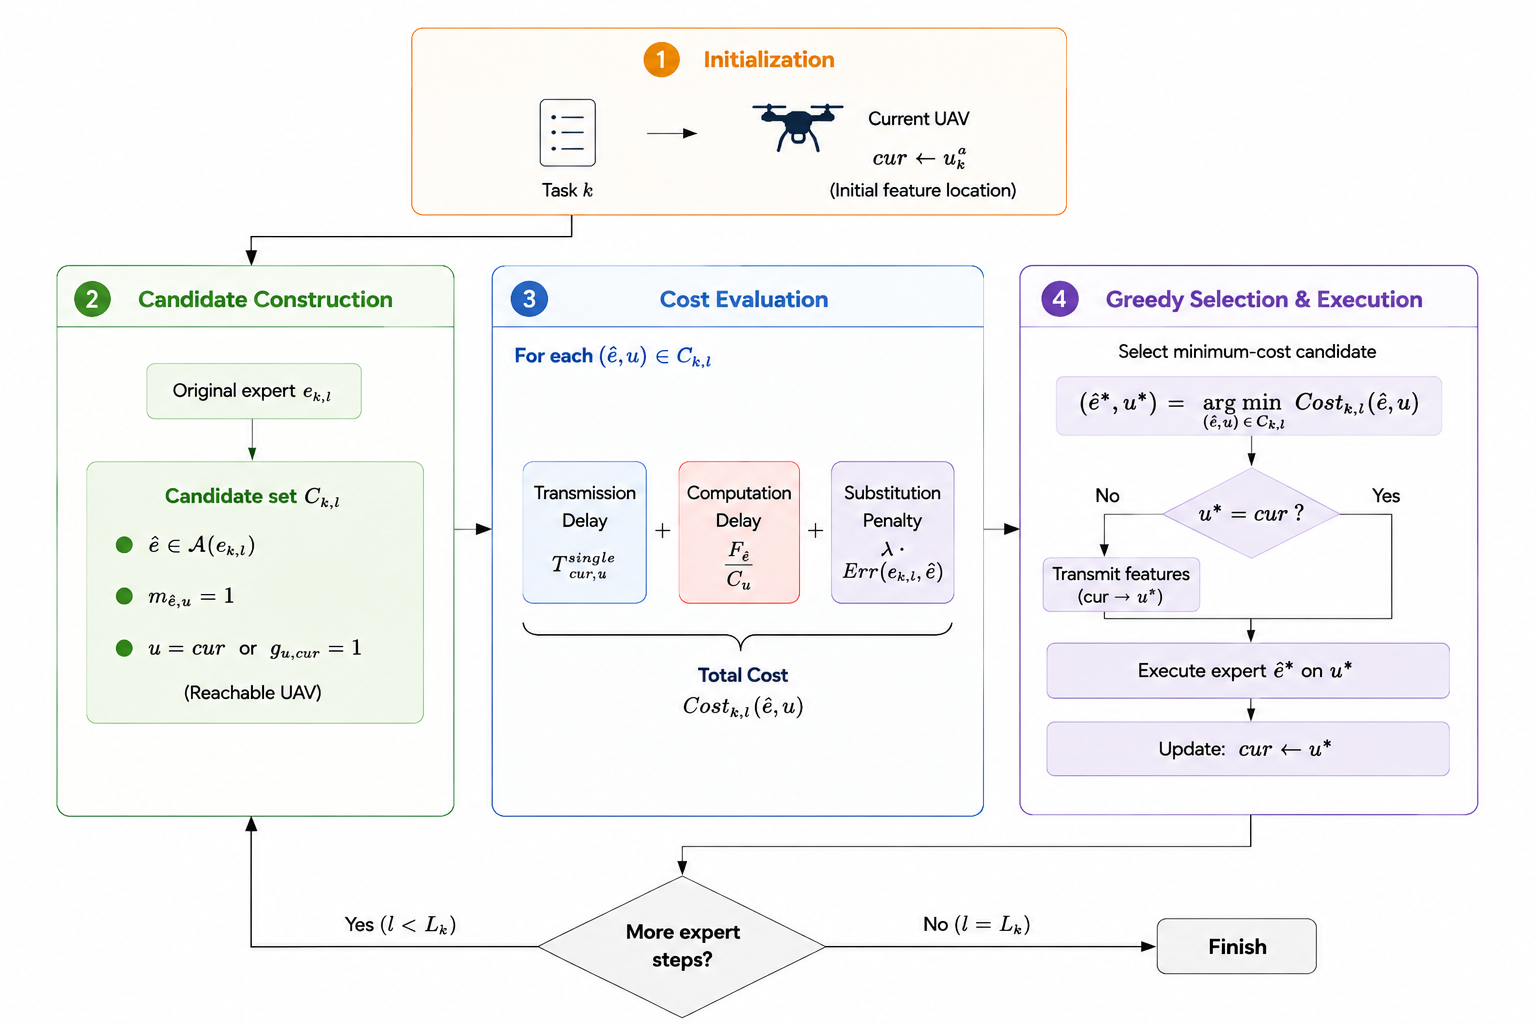
\includegraphics[width=1.05\columnwidth]{scheduling.png}
    \caption{Lightweight inference scheduling.}
    \label{fig:scheduling}
\end{figure}

For each task \(k\), inference begins at its default access UAV after the shared attention and gating layers are executed, 
${\rm cur} \leftarrow u_k^a$,
where \({\rm cur}\) tracks the UAV currently holding the intermediate features and is updated after each cross-UAV transmission.

For the \(l\)-th expert step of task \(k\), let \(e_{k,l}\) be the expert selected by the gating network. The candidate set of execution pairs \((\hat{e}, u)\) consists of all deployed experts \(\hat{e} \in \mathcal{A}(e_{k,l})\) that are either local to the current or reachable UAV, and whose computation requirement does not exceed the remaining compute budget of the target UAV, i.e.,
\begin{equation}
\begin{aligned}
\mathcal{C}_{k,l} = \{ (\hat{e}, u) \mid &\hat{e} \in \mathcal{A}(e_{k,l}),\ m_{\hat{e},u}=1, \\
&u = {\rm cur}\ \text{or}\ g_{{\rm cur},u}=1,\ \tilde{C}_u \ge F_{\hat{e}} \}.
\end{aligned}
\end{equation}
Here, \(\hat{e}\) may be the originally required expert \(e_{k,l}\) or any sufficiently similar deployed substitute, and \(u\) is the candidate execution UAV.
The cost of executing expert \(\hat{e}\) on UAV \(u\) at step \(l\) is defined as
\begin{equation}\label{e35}
\begin{aligned}
\mathrm{Cost}_{k,l}(\hat{e}, u) &= T_{{\rm cur},u}^{\mathrm{single}}(S_{k,l-1}^{\mathrm{mid}}) \\
&\quad + \frac{F_{\hat{e}}}{C_u} + \lambda \cdot \mathrm{Err}(e_{k,l}, \hat{e}),
\end{aligned}
\end{equation}
where \(T_{{\rm cur},u}^{\mathrm{single}}(S_{k,l-1}^{\mathrm{mid}})\) is the single-hop transmission delay from the current UAV to UAV \(u\) (zero if \(u = {\rm cur}\)); \(F_{\hat{e}}/C_u\) is the computation delay on UAV \(u\); \(\mathrm{Err}(e_{k,l}, \hat{e}) = 1 - \mathrm{Sim}(e_{k,l}, \hat{e})\) is the approximation error incurred by using a substitute (zero when \(\hat{e} = e_{k,l}\)); \(\lambda > 0\) is a penalty weight that trades off execution latency against substitution error.

At each step, the scheduler greedily selects the minimum-cost candidate:
\begin{equation}
(\hat{e}^*, u^*) = \arg\min_{(\hat{e},u) \in \mathcal{C}_{k,l}} \mathrm{Cost}_{k,l}(\hat{e}, u).
\end{equation}
If \(u^* \neq {\rm cur}\), the intermediate features are transmitted from \({\rm cur}\) to \(u^*\) over a single-hop link. The expert \(\hat{e}^*\) is then executed on \(u^*\), after which the current location is updated as \({\rm cur} \leftarrow u^*\).

This per-step greedy selection, together with the candidate construction rules, ensures that each expert layer is executed on exactly one UAV while satisfying the single-hop transmission and per-UAV compute capacity constraints.
% ==============================================================
\section{Simulation Results}
\label{sec:eval}
% ==============================================================



%为验证第~\ref{sec:design}~节提出的 AeroMoE 设计，本文实现了一个Python 仿真评估管线。该仿真器按照第~\ref{sec:system}~节的准静态UAV 边缘网络模型生成 UAV 拓扑、空地接入链路、UAV-UAV 单跳链路、推理任务和候选专家集合，并按照第~\ref{sec:design}~节的分阶段流程依次执行任务需求建模、相似候选专家构造、通信感知部署评分、动态贪心专家部署和逐层推理调度。所有结果均在多个随机种子下重复运行，并报告平均值和标准差。Fig.~\ref{fig:simulation} 给出了仿真场景图

% \begin{figure}[ht]
%   %\centering
%   \includegraphics[width=0.92\columnwidth]{photo/simulation.png}
%   \caption{场景图}
%   \label{fig:simulation}
% \end{figure}



%\textbf{UAV 与通信设置。}
% 仿真场景由多个准静态 UAV 组成。每个 UAV 具有三维位置、可用计算能力$C_u$、可用于存放专家参数的内存容量 $M_u$ 以及发射功率。空地接入链路和 UAV-UAV 协同链路均根据距离相关路径损耗计算信噪比，并通过阈值$\rho_{\mathrm{th}}$ 判断链路是否可用。若 UAV $u$ 与 UAV $v$ 之间满足单跳连通条件，则按带宽和信噪比计算传输速率 $R_{u,v}$；否则该 UAV 对不能在当前调度步骤中直接传输中间特征。
% %\pdfcomment{做一个场景图}
% %\textbf{场景生成。}
% 为模拟 UAV 边缘网络中的区域性任务需求，本文采用受控随机热点场景。仿真区域大小为 $240\,\mathrm{m}\times240\,\mathrm{m}$，4 个 UAV 分别部署在四个服务区域附近，其水平位置在区域中心周围加入小幅随机扰动，高度在$70$--$90$\,m 范围内随机采样。不同 UAV 的计算能力和内存容量也随机采样，以体现准静态网络中的资源异构性。任务围绕各 UAV 形成局部热点，每个热点区域具有不同的专家需求分布，用于模拟灾害监测、低空巡检等场景中不同地理区域产生不同类型推理请求的情况。

% 专家集合包含 8 个专家，其中部分专家具有较大的内存占用和计算量，用于表示任务原本需要的主要专家；另一些专家被构造为与主要专家权重向量相近的轻量级替代专家。该设置一方面引入内存压力，使所有原始专家无法简单地全部复制到每个 UAV 上；另一方面为第~\ref{sec:similarity_candidate}~节的相似替代机制提供可验证的候选结构。所有随机量均由固定随机种子控制，实验报告多个种子下的平均结果，以减少单一场景偶然性对结论的影响。

% %\textbf{任务与专家设置。}
% 每个任务包含地面位置、输入大小 $S_k^{\mathrm{in}}$、输出大小$S_k^{\mathrm{out}}$、逐层中间特征大小 $S_{k,l}^{\mathrm{mid}}$、任务权重$\omega_k$ 以及由 gating 决定的专家执行序列 $\mathbf{e}_k$。每个专家具有内存占用 $W_e$、单次前向计算量 $F_e$ 和用于计算余弦相似度的权重向量。在没有真实 gating score 的情况下，任务对专家的需求强度 $q_{k,r}$由专家在任务执行序列中的出现次数统计。默认参数设置为$\alpha=0.4$、$\beta=0.25$、$\gamma=0.2$、$\mu=0.15$、$\eta=0.5$、$\nu=0.3$、$\eta_{\mathrm{red}}=0.5$、$\lambda=0.1$，相似度阈值默认为 $\xi=0.7$。


% 为便于复现实验，表~\ref{tab:simulation_parameters} 总结了默认仿真场景和无线信道参数，表~\ref{tab:task_expert_parameters} 给出了任务与专家池设置，表~\ref{tab:algorithm_sweep_parameters}列出了算法超参数以及敏感性、扩展性实验中的参数扫描范围。
\subsection{Simulation Setup}
\label{sec:setup}
The simulation considers a quasi-static UAV edge network consisting of multiple UAVs. Each UAV is characterized by its three-dimensional position, computation capability \(C_u\), memory capacity \(M_u\) available for expert parameters, and transmit power. %Both air-to-ground access links and UAV-to-UAV links are modeled using distance-dependent path loss. The signal-to-noise ratio is computed accordingly, and a link is considered available only if its SNR exceeds a predefined threshold \(\rho_{\rm th}\). 
When two UAVs satisfy the connectivity condition, the intermediate feature transmission is permitted; otherwise, direct intermediate feature transmission between them is not permitted in the current scheduling step.
To emulate spatially heterogeneous task demands typical in UAV edge scenarios, we adopt a controlled random hotspot setup. The simulation area is \(240\,\mathrm{m} \times 240\,\mathrm{m}\), with 4 UAVs deployed near the centers of 4 service regions. Their horizontal positions are perturbed with small random offsets, and their altitudes are uniformly sampled between 70 m and 90 m. The computing power and memory capacities of the UAVs are also randomly sampled to reflect resource heterogeneity. Tasks are generated as localized hotspots around each UAV, with distinct expert demand distributions across regions. This setup mimics realistic applications such as disaster monitoring and low-altitude inspection, where different geographic areas generate different types of inference requests.

The expert pool contains eight experts. Some experts have large memory footprints and high computing requirements, representing the primary experts originally required by tasks. Others are constructed as lightweight substitutes whose weight vectors are similar to those of the primary experts. This configuration creates realistic memory pressure, preventing all original experts from being replicated on every UAV, while also providing a verifiable structure for evaluating the similarity-based substitution mechanism. All random variables are controlled by fixed random seeds, and experimental results are averaged over multiple seeds to reduce the impact of particular random realizations.

Each task is defined by its ground location, input size \(S_k^{\rm in}\), output size \(S_k^{\rm out}\), per-layer intermediate feature sizes \(S_{k,l}^{\rm mid}\), weight \(\omega_k\), and expert execution sequence \(\mathbf{e}_k\) determined by the gating network. Each expert is characterized by its memory footprint \(W_e\), per-forward computation requirement \(F_e\), and weight vector used for cosine similarity computation. When gating scores are unavailable, the demand intensity \(q_{k,r}\) of expert \(r\) in task \(k\) is computed from its occurrence count in the expert sequence of task \(k\).

The default algorithm parameters are set as follows: \(\alpha=0.4\), \(\beta=0.25\), \(\gamma=0.2\), \(\mu=0.15\), \(\eta=0.5\), \(\nu=0.3\), \(\eta_{\rm red}=0.5\), \(\lambda=0.1\), and similarity threshold \(\xi=0.7\). For reproducibility, the default simulation and wireless channel parameters are summarized in Table~\ref{tab:simulation_parameters}, the task and expert pool configurations are listed in Table~\ref{tab:task_expert_parameters}, and the algorithm hyperparameters along with their ranges used in sensitivity and scalability studies are provided in Table~\ref{tab:algorithm_sweep_parameters}.

\begin{table}[!t]
  \centering
  \caption{SIMULATION SCENARIO AND WIRELESS SETTINGS.}
  \label{tab:simulation_parameters}
  \footnotesize
  \setlength{\tabcolsep}{3pt}
  \renewcommand{\arraystretch}{1.12}
  \begin{tabular}{@{}>{\raggedright\arraybackslash}p{0.34\columnwidth}
                  >{\raggedright\arraybackslash}p{0.58\columnwidth}@{}}
    \toprule
    Item & Setting \\
    \midrule
    \multicolumn{2}{@{}l}{\textit{Scenario scale}} \\
    Scenario & Controlled random hotspot UAV scenario \\
    Random seeds & $\{0,1,2,3,4\}$ \\
    Area & $240\,\mathrm{m}\times240\,\mathrm{m}$ \\
    UAVs / tasks / experts & $U=4$, $K=40$, $E=8$ \\
    Expert vector dimension & 64 \\
    \addlinespace[1pt]
    \midrule
    \multicolumn{2}{@{}l}{\textit{UAV resources}} \\
    Base positions & $(60,60)$, $(180,60)$, $(60,180)$, $(180,180)$ \\
    Position perturbation & $x,y\sim\mathcal{U}[-10,10]$ m; $H\sim\mathcal{U}[70,90]$ m \\
    Computing capability $C_u$ & $\mathcal{U}[8,11]$ GFLOP/s \\
    Memory capacity $M_u$ & $\mathcal{U}[850,1050]$ MB \\
    UAV transmit power $P_u$ & $\mathcal{U}[10,14]$ W \\
    \addlinespace[1pt]
    \midrule
    \multicolumn{2}{@{}l}{\textit{Wireless channel}} \\
    Reference gain $\beta_0$ & 1 \\
    Path-loss exponent & 2.5 \\
    Noise density $N_0$ & $10^{-12}$ W/Hz \\
    Bandwidth $B$ & 20 MHz \\
    SNR threshold $\gamma_{\mathrm{th}}$ & 5 \\
    Ground transmit power & 5 W \\
    \bottomrule
  \end{tabular}
\end{table}

\begin{table}[!t]
  \centering
  \caption{TASK AND EXPERT SPECIFICATIONS.}
  \label{tab:task_expert_parameters}
  \footnotesize
  \setlength{\tabcolsep}{3pt}
  \renewcommand{\arraystretch}{1.12}
  \begin{tabular}{@{}>{\raggedright\arraybackslash}p{0.34\columnwidth}
                  >{\raggedright\arraybackslash}p{0.58\columnwidth}@{}}
    \toprule
    Item & Setting \\
    \midrule
    \multicolumn{2}{@{}l}{\textit{Expert pool}} \\
    Original experts $E_0$--$E_3$ & $W_e\sim\mathcal{U}[620,760]$ MB, $F_e\sim\mathcal{U}[1.0,1.35]$ GFLOP \\
    Substitute experts $E_4$--$E_6$ & $W_e\sim\mathcal{U}[220,320]$ MB, $F_e\sim\mathcal{U}[0.35,0.52]$ GFLOP \\
    Auxiliary expert $E_7$ & $W_e\sim\mathcal{U}[280,380]$ MB, $F_e\sim\mathcal{U}[0.50,0.70]$ GFLOP \\
    Similar pairs & $(E_0,E_4)$, $(E_1,E_5)$, $(E_2,E_6)$ \\
    Similarity noise scale & $\mathcal{U}[0.06,0.10]$ \\
    \addlinespace[1pt]
    \midrule
    \multicolumn{2}{@{}l}{\textit{Task profile}} \\
    Number of layers & $\mathcal{U}\{2,3,4\}$ \\
    Input size $S_k^{\mathrm{in}}$ & $\mathcal{U}[1.0,2.2]$ Mbit \\
    Output size $S_k^{\mathrm{out}}$ & $\mathcal{U}[10,25]$ kbit \\
    Mid-feature size $S_{k,l}^{\mathrm{mid}}$ & First value $\mathcal{U}[0.8,1.4]$ Mbit, then multiplied by $0.9^l$ \\
    Task priority $\omega_k$ & $\mathcal{U}[0.8,1.4]$ \\
    Hotspot spread & Gaussian offset, $\sigma=12$ m \\
    \addlinespace[1pt]
    \midrule
    \multicolumn{2}{@{}l}{\textit{Hotspot expert distributions}} \\
    UAV 0 & experts $(0,1,3,2)$, probabilities $(0.75,0.15,0.07,0.03)$ \\
    UAV 1 & experts $(1,3,0,2)$, probabilities $(0.75,0.15,0.07,0.03)$ \\
    UAV 2 & experts $(2,0,3,1)$, probabilities $(0.75,0.15,0.07,0.03)$ \\
    UAV 3 & experts $(0,2,1,3)$, probabilities $(0.48,0.48,0.02,0.02)$ \\
    \bottomrule
  \end{tabular}
\end{table}

\begin{table}[!t]
  \centering
  \caption{ALGORITHM PARAMETERS AND SWEEP SETTINGS.}
  \label{tab:algorithm_sweep_parameters}
  \footnotesize
  \setlength{\tabcolsep}{3pt}
  \renewcommand{\arraystretch}{1.12}
  \begin{tabular}{@{}>{\raggedright\arraybackslash}p{0.34\columnwidth}
                  >{\raggedright\arraybackslash}p{0.58\columnwidth}@{}}
    \toprule
    Item & Setting \\
    \midrule
    \multicolumn{2}{@{}l}{\textit{Default algorithm parameters}} \\
    Similarity threshold & $\xi=0.7$ \\
    Placement score weights & $\alpha=0.4$, $\beta=0.25$, $\gamma=0.2$, $\mu=0.15$ \\
    Remote-demand weight & $\eta=0.5$ \\
    Redundancy weights & $\nu=0.3$, $\eta_{\mathrm{red}}=0.5$ \\
    Scheduling penalty & $\lambda=0.1$ \\

    Expert copy limit & One copy per expert in the default scenario \\
    \addlinespace[1pt]
    \midrule
    \multicolumn{2}{@{}l}{\textit{Sensitivity studies}} \\
    Similarity threshold & $\xi\in\{0.5,0.6,0.7,0.8,0.9,1.0\}$ \\
    UAV memory scale & $\{0.9,1.0,\ldots,1.4\}$ \\
    Mid-feature scale & $\{0.4,0.6,\ldots,2.0\}$ \\
    \addlinespace[1pt]
    \midrule
    \multicolumn{2}{@{}l}{\textit{Scalability studies}} \\
    UAV count & $U\in\{4,6,\ldots,20\}$; $K=60$, $E=8$ \\
    Task count & $K\in\{20,30,\ldots,100\}$; $U=10$, $E=8$ \\
    Expert count & $E\in\{8,10,\ldots,24\}$; $U=10$, $K=80$ \\
    
    \bottomrule
  \end{tabular}
\end{table}


\subsection{Baselines and Metrics}
\label{sec:baselines_metrics}

% 为隔离 AeroMoE 各设计模块的作用，本文比较以下方法：
% \begin{itemize}
%   \item \textbf{Proposed}: 完整 AeroMoE 方法，包含相似候选构造、有效需求扩展、通信感知评分、覆盖预部署、动态冗余贪心部署和逐层调度。
%   \item \textbf{Random Placement}: 在满足内存约束的条件下随机部署候选专家，然后使用与 Proposed 相同的逐层单跳调度器。
%   \item \textbf{Importance}: 按专家的全局有效需求排序部署，忽略通信可达性、UAV 算力差异和网络位置收益。
%   \item \textbf{No-Sim}: 关闭相似专家替代机制，仅允许部署和执行任务原本需要的专家。
% \end{itemize}

% 主要评估指标为端到端总延迟 $D_{\mathrm{total}}$，并进一步统计接入延迟、专家计算延迟、UAV-UAV 传输延迟和结果回传延迟的分解项。为分析相似替代机制的作用，本文还统计替代专家的使用次数；为验证鲁棒性，进一步对相似阈值 $\xi$、中间特征大小和 UAV 内存容量进行敏感性分析。最后，本文从UAV 数量、任务数量和专家池规模三个维度评估方法的扩展性。
To isolate the contribution of each design component in AeroMoE, we compare the following schemes.

\begin{itemize}
    \item \textbf{Proposed}: The complete AeroMoE framework, including similarity-aware candidate construction, effective demand extension, communication-aware scoring, coverage-aware pre-deployment, dynamic redundancy-penalized greedy placement, and per-layer scheduling.
    \item \textbf{Random Placement}: Candidate experts are randomly deployed subject to memory constraints, followed by the same per-layer single-hop scheduler used in the Proposed scheme.
    \item \textbf{Importance}: Experts are deployed in descending order of their global effective demand, without considering communication connectivity, UAV computation heterogeneity, or network position benefits.
    \item \textbf{No-Sim}: Similarity-based expert substitution is disabled; only originally required experts may be deployed and executed.
\end{itemize}

The primary performance metric is the total latency \(D_{\mathrm{total}}\). We further decompose the latency into access delay, expert computation delay, UAV-UAV transmission delay, and result return delay. To evaluate the effectiveness of similarity-based substitution, we also report the number of times substitute experts are used during inference. For robustness analysis, we conduct sensitivity studies with respect to the similarity threshold \(\xi\), intermediate feature size, and UAV memory capacity. Finally, we evaluate the scalability of AeroMoE by varying the number of UAVs, the number of tasks, and the size of the expert pool.

\subsection{Performance Analysis}
\label{sec:e2e_delay}
%\pdfcomment{q1：图不知道为啥在下边。。q2：senstivity的图还需要改改，但是没思路（是直接用x，还是从0.8开始}
% Fig.~\ref{fig:total_delay} 给出了各方法在多随机种子下的平均端到端延迟。
% Proposed 的平均总延迟为 $9878.9$\,ms，低于 Random Placement 的
% $13014.9$\,ms 和 Importance 的 $12527.7$\,ms；与 Importance 相比，
% Proposed 将平均延迟降低约 $21.1\%$。No-Sim 的平均总延迟达到
% $19107.5$\,ms，说明在内存受限 UAV 网络中，若不允许相似专家替代，
% 系统往往需要使用更差的部署和执行路径，导致端到端延迟显著升高。
\subsubsection{End-to-End Delay Performance}
Fig.~\ref{fig:total_delay} shows the average end-to-end latency of different methods across multiple random seeds.Compared with Random Placement, Importance, and No-Sim, AeroMoE reduces the average end-to-end latency by 24.1\%, 21.1\%, and 48.3\%, respectively. The Proposed scheme achieves an average latency of 9878.9 ms, outperforming Random Placement (13014.9 ms) and Importance (12527.7 ms). No-Sim yields the highest average latency of 19107.5 ms, indicating that disabling similarity-based substitution forces the system to adopt suboptimal deployment and execution paths under tight memory constraints.

\begin{figure}[t]
  %\centering
  
\includegraphics[width=0.98\columnwidth]{fig1_total_delay.pdf}
  \caption{Average end-to-end latency comparison of different expert deployment methods.}
  \label{fig:total_delay}
\end{figure}

%该结果表明，AeroMoE 的收益并非来自单一因素，而是来自需求驱动候选构造、通信感知部署评分和动态冗余贪心选择的共同作用。Random Placement 缺乏需求和拓扑信息，容易把专家部署到通信或计算条件不理想的 UAV 上；Importance 只关注全局需求，不能区分专家部署在不同 UAV 上的通信收益；No-Sim 则失去了相似专家带来的候选扩展和内存节省能力。
These results indicate that the performance gains of AeroMoE stem from the joint effect of demand-driven candidate construction, communication-aware placement scoring, and dynamic redundancy-penalized greedy selection, rather than from any single component. Random Placement lacks awareness of task demand and network topology, often placing experts on UAVs with unfavorable communication or computation conditions. Importance considers only global demand and fails to account for the communication benefits of deploying experts on different UAVs. No-Sim, by disabling similarity-based substitution, loses the ability to expand the candidate set and reduce memory pressure through expert reuse.
\subsubsection{Delay Breakdown}

% Fig.~\ref{fig:delay_breakdown} 展示了端到端延迟的组成。各方法的接入延迟和回传延迟差异较小，因为它们共享相同的任务接入规则和无线链路模型；主要差异来自专家计算延迟和 UAV-UAV 中间特征传输延迟。Proposed 的平均计算延迟为 $171.8$\,ms，低于 Random Placement 的 $233.8$\,ms、Importance 的 $231.1$\,ms 和 No-Sim 的 $394.8$\,ms；平均传输延迟为$40.2$\,ms，也低于 Random Placement 的 $56.5$\,ms、Importance 的$47.1$\,ms 和 No-Sim 的 $48.0$\,ms。

\begin{figure}[!t]
  \centering
  
\includegraphics[width=0.98\columnwidth]{fig2_delay_breakdown.pdf}
  \caption{End-to-end latency breakdown. AeroMoE reduces both computation and transmission overhead through communication-aware deployment and per-layer scheduling.}
  \label{fig:delay_breakdown}
\end{figure}

% 该分解结果与第~\ref{sec:placement_scoring}~节的评分设计一致。$A(e,u)$ 倾向于将专家部署到能够服务本地和单跳邻域需求的位置，从而降低跨 UAV 传输；$B(e,u)$ 倾向于将计算量较大的专家部署到算力较强的 UAV 上；动态冗余惩罚进一步避免在同一区域重复部署功能高度重叠的专家，使有限内存被用于更有增益的候选。图中 No-Sim 的计算延迟明显高于其他方法，说明在不能使用相似替代时，任务更容易被迫执行原始且开销较大的专家；Random Placement 和 Importance 虽然可以使用替代专家，但缺少完整的通信和算力匹配机制，因此计算与传输两项开销仍高于 Proposed。
Fig.~\ref{fig:delay_breakdown} presents the breakdown of end-to-end latency. The access and return delays are comparable across all methods, as they share the same task assignment policy and wireless channel model. The main differences lie in expert computation delay and UAV-UAV transmission delay. The Proposed scheme achieves an average computation delay of 171.8 ms, which is lower than Random Placement (233.8 ms), Importance (231.1 ms), and No-Sim (394.8 ms). Its average transmission delay is 40.2 ms, also lower than Random Placement (56.5 ms), Importance (47.1 ms), and No-Sim (48.0 ms).

These results are consistent with the design of the placement scoring mechanism in Section~\ref{sec:placement_scoring}. The term $A(e,u)$ encourages the placement of experts in locations that can serve both local and single-hop neighboring demands, thereby reducing cross-UAV transmissions. The term $B(e,u)$ favors assigning computation-intensive experts to UAVs with higher processing capability. In addition, the dynamic redundancy penalty prevents the repeated deployment of functionally similar experts in the same region, allowing limited memory to be allocated to higher-gain candidates. No-Sim exhibits significantly higher computation delay because it cannot exploit similarity-based substitution and is forced to execute more expensive original experts. Although Random Placement and Importance can utilize substitute experts, they lack a comprehensive mechanism that jointly considers communication and computation conditions, resulting in higher computation and transmission overheads compared with the Proposed scheme.
\subsubsection{Similarity Substitution Analysis}
\label{sec:substitution_analysis}

% Fig.~\ref{fig:substitutions} 统计了不同方法中替代专家的使用次数。Proposed 平均产生 $114.8$ 次替代执行，高于 Random Placement 的$85.8$ 次和 Importance 的 $89.6$ 次；No-Sim 的替代次数为 $0$。这说明 AeroMoE 不仅在部署阶段把相似专家作为候选，也在在线推理调度阶段实际利用这些替代专家来降低传输和计算代价。

\begin{figure}[!t]
  \centering
  
\includegraphics[width=0.98\columnwidth]{fig3_substitutions.pdf}
  \caption{Number of substitute expert usages. The Proposed scheme utilizes similar experts more effectively to cover originally required demands.}
  \label{fig:substitutions}
\end{figure}

% 相似替代机制的作用可以从两个层面解释。首先，在部署阶段，$\mathcal{A}(r)$ 将原始需求专家扩展为可替代候选，$\mathrm{Demand}^{\mathrm{eff}}$使替代专家继承原始专家的部分需求，从而在内存受限时提供更大的部署选择空间。其次，在调度阶段，式~(\ref{e35}) 中的误差项$\lambda(1-\mathrm{Sim})$ 防止系统无约束地选择低质量替代专家，使延迟收益
% 和替代误差之间保持可控折中。
Fig.~\ref{fig:substitutions} shows the number of times substitute experts are used during inference. The Proposed scheme utilizes substitute experts 114.8 times on average, which is higher than Random Placement (85.8 times) and Importance (89.6 times). No-Sim, as expected, uses no substitutes. These results demonstrate that AeroMoE not only includes similar experts as deployment candidates but also actively leverages them during online scheduling to reduce both transmission and computation costs.

The benefits of similarity-based substitution arise at two stages. In the deployment stage, the substitutable set \(\mathcal{A}(r)\) expands the candidate pool beyond originally required experts, while the effective demand \(\mathrm{Demand}^{\mathrm{eff}}\) allows substitute experts to inherit part of the original demand. This provides greater deployment flexibility under memory constraints. In the scheduling stage, the error penalty term \(\lambda(1 - \mathrm{Sim})\) in the cost function prevents the selection of low-quality substitutes, maintaining a controlled trade-off between latency reduction and approximation error.
\subsubsection{Sensitivity Analysis}
\label{sec:sensitivity}

% Fig.~\ref{fig:sensitivity_xi} 展示了相似度阈值 $\xi$ 对系统性能的影响。当 $\xi$ 较低时，候选集合包含更多替代专家，系统具有更大的部署灵活性；当 $\xi$ 提高时，低相似度替代被过滤，候选空间收缩。图中 Proposed 在$\xi=0.5$--$0.9$ 范围内始终低于各基线，说明较低阈值扩大了可选空间，但并不会使系统无约束地大量使用低质量替代专家。这是因为候选替代仍需满足相似度条件，且在线调度代价中包含式~(\ref{e35}) 的替代误差惩罚，从而限制了低相似度替代的使用。

% 当 $\xi=1.0$ 时，只有与原始专家完全相同的专家能够进入候选集合，相似替代事实上被关闭。此时 Proposed 退化为精确匹配策略，因此其延迟明显上升并接近 No-Sim。Random Placement 和 Importance 在该点也不能获得更低延迟，因为它们的部署策略分别依赖随机放置或全局需求排序，不能像Proposed 那样结合覆盖预部署、通信感知评分和动态冗余贪心来优化精确专家
% 的部署位置。
Fig.~\ref{fig:sensitivity_xi} shows the impact of the similarity threshold \(\xi\) on system performance. A lower \(\xi\) enlarges the candidate set by including more substitute experts, thereby increasing deployment flexibility. As \(\xi\) increases, weakly similar substitutes are filtered out and the candidate space shrinks. The Proposed scheme consistently outperforms all baselines for \(\xi \in [0.5, 0.9]\). This indicates that a moderate threshold expands the available options without allowing the excessive use of low-quality substitutes. The similarity requirement itself, combined with the approximation error penalty in the scheduling cost function, effectively prevents the selection of poor substitutes.

When \(\xi = 1.0\), only identical experts are admitted into the candidate set, effectively disabling similarity-based substitution. In this case, the Proposed scheme degenerates into an exact-matching strategy, and its latency rises sharply to approach that of No-Sim. Random Placement and Importance also fail to achieve lower latency at this point, as their deployment strategies rely solely on randomness or global demand ordering and lack the coordinated mechanisms of coverage pre-deployment, communication-aware scoring, and dynamic redundancy control that enable more effective placement of exact experts.
%\pdfcomment{相似度阈值这个图不知道为啥少了一部分，在文件夹里看是正常的}
\begin{figure}[!t]
  \centering
  
\includegraphics[width=0.98\columnwidth,trim=0 0 0 0,clip]{fig4_sensitivity_xi.pdf}
  \caption{Sensitivity analysis with respect to the similarity threshold $\xi$.}
  \label{fig:sensitivity_xi}
\end{figure}

%Fig.~\ref{fig:sensitivity_mid} 进一步分析中间特征大小的影响。随着$S^{\mathrm{mid}}$ 增大，跨 UAV 传输开销在端到端延迟中占比上升，各方法延迟均随之增加，但 Proposed 的增长幅度最小，并在全部特征规模下保持最低延迟。其原因是 AeroMoE 在部署评分中显式考虑单跳可达性和链路速率，使高需求专家更倾向于部署在可达性较好的 UAV 上；同时，相似替代机制增加了可选执行位置，减少了大尺寸中间特征在低速链路上的传输。因此在通信压力增大时，Proposed 仍能保持较低延迟。

\begin{figure}[!t]
  \centering
  
\includegraphics[width=0.98\columnwidth]{fig5_sensitivity_mid_size.pdf}
  \caption{Impact of intermediate feature size on end-to-end latency.}
  \label{fig:sensitivity_mid}
\end{figure}
%\pdfcomment{要解释说明，}
%Fig.~\ref{fig:sensitivity_memory} 给出了 UAV 内存容量变化时的性能趋势。

%No-Sim 和非通信感知方法也更容易受到专家覆盖不足和低质量部署位置的影响。AeroMoE 通过覆盖预部署和相似替代优先保证原始需求可服务，再利用动态贪心在剩余内存上补充高收益专家。随着内存容量增加，各方法均获得更多部署空间，但 AeroMoE 仍保持较低延迟，表明其收益不仅来自部署更多专家，也来自更合理的专家-UAV 匹配。图中 Random Placement 和 Importance 在内存从紧张变为充足时延迟下降较明显，说明它们更依赖额外容量弥补部署选择不足；相比之下，Proposed 在可行区间内变化更平稳，表明其在有限内存下已经能够优先选择高收益专家和合适部署位置。No-Sim 随内存增加改善有限，进一步说明仅增加容量不能替代相似候选带来的部署弹性。
Fig.~\ref{fig:sensitivity_mid} further examines the impact of intermediate feature size. As \(S^{\mathrm{mid}}\) increases, the proportion of cross-UAV transmission delay in the end-to-end latency rises, causing all methods to experience higher latency. However, the Proposed scheme exhibits the smallest increase and maintains the lowest latency across all feature sizes. This robustness stems from two aspects of the design. First, the communication-aware placement scoring explicitly accounts for single-hop reachability and link rates, encouraging the deployment of high-demand experts on well-connected UAVs. Second, similarity-based substitution expands the set of feasible execution locations, reducing the need to transmit large intermediate features over low-rate links.

Fig.~\ref{fig:sensitivity_memory} shows the performance trends as UAV memory capacity varies. As memory becomes more abundant, all methods gain additional deployment space and achieve lower latency. Nevertheless, the Proposed scheme consistently maintains the lowest latency and exhibits the most stable performance. This advantage arises because AeroMoE uses coverage pre-deployment and similarity substitution to ensure that originally required experts can be served, while the dynamic greedy algorithm allocates remaining memory to high-gain placements. In contrast, Random Placement and Importance benefit more significantly from increased memory, indicating that they rely more heavily on extra capacity to compensate for suboptimal deployment decisions. No-Sim shows limited improvement with larger memory budgets, confirming that simply increasing capacity cannot fully substitute for the deployment flexibility provided by similarity-based candidate expansion.

\begin{figure}[!t]
  \centering
  
\includegraphics[width=0.98\columnwidth]{fig6_sensitivity_memory.pdf}
  \caption{Impact of UAV memory capacity on end-to-end latency and deployment scale.}
  \label{fig:sensitivity_memory}
\end{figure}

\subsubsection{Scalability Analysis}
\label{sec:scalability}

%除上述参数敏感性外，本文进一步考察系统规模变化时的性能。Fig.~\ref{fig:scale_uav}仅增加 UAV 数量，并保持任务和专家设置不变。随着 UAV 数量从 4 增加到20，Proposed 的平均单任务延迟整体保持在较低水平，并从约 $175$\,ms降至约 $162$\,ms，始终低于所有基线。增加 UAV 会带来更多可部署位置和更短的平均接入距离，但只有在部署策略能够同时利用任务需求、单跳连通性和 UAV 计算异构性时，这些额外资源才能稳定转化为延迟收益。Random 和 Importance 在 UAV 较少时容易受到部署位置不匹配影响；No-Sim 虽然也受益于更多 UAV，但由于缺乏替代专家带来的内存弹性，延迟仍显著高于其他方法。图中 Proposed 曲线只出现小幅波动，说明 UAV 数量变化带来的拓扑随机性不会破坏其稳定优势。
Beyond parameter sensitivity, we further evaluate the scalability of AeroMoE with respect to system size. Fig.~\ref{fig:scale_uav} shows the results when increasing the number of UAVs while keeping the number of tasks and experts fixed. As the number of UAVs grows from 4 to 20, the average per-task latency of the Proposed scheme remains low and decreases slightly from approximately 175 ms to 162 ms, consistently outperforming all baselines. Although a larger number of UAVs provides more deployment options and shorter average access distances, these additional resources translate into stable latency gains only when the deployment strategy jointly exploits task demand, single-hop connectivity, and UAV computation heterogeneity. Random Placement and Importance suffer more from mismatched deployment locations when the number of UAVs is small, while No-Sim, despite benefiting from more UAVs, still exhibits significantly higher latency due to the lack of memory flexibility from similarity-based substitution. The Proposed curve shows only minor fluctuations, indicating that topological randomness introduced by varying UAV counts does not undermine its performance advantage.

\begin{figure}[!t]
  \centering
  \IfFileExists{fig7_uav_count.pdf}{%
    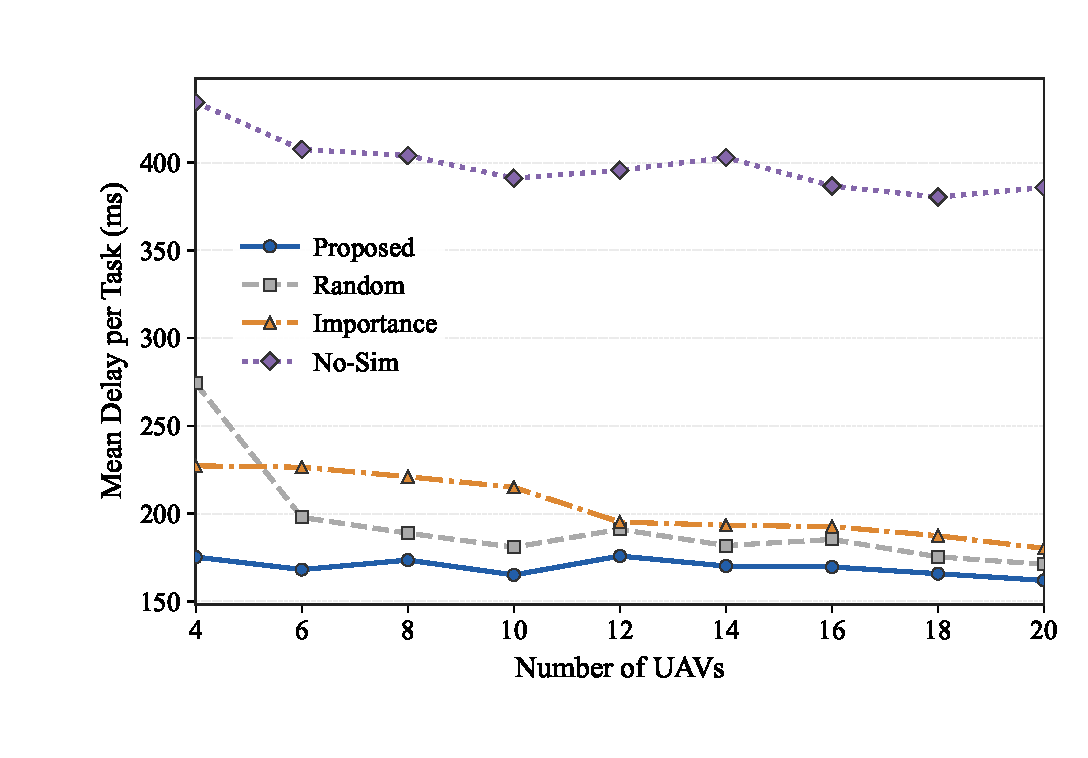
\includegraphics[width=0.98\columnwidth]{fig7_uav_count.pdf}%
  }{%
    \fbox{\parbox{0.88\columnwidth}{\centering Missing figure file:\\
    fig7\_uav\_count.pdf}}%
  }
  \caption{Scalability with respect to the number of UAVs.}
  \label{fig:scale_uav}
\end{figure}

%Fig.~\ref{fig:scale_task} 仅增加任务数量，并报告平均单任务延迟。当任务数从 20 增加到 100 时，各方法的平均单任务延迟整体保持稳定，说明任务数量增加主要改变需求统计和调度次数，而不会直接破坏单跳执行结构。Proposed 在所有任务规模下保持最低延迟，表明需求驱动的有效专家建模能够从更多任务样本中提取更稳定的部署偏好。图中 No-Sim 始终处于最高延迟，说明在任务规模增加时，缺少替代专家仍会持续放大原始专家覆盖和执行路径受限带来的开销；Random Placement 和 Importance 则因部署策略对局部需求和链路条件利用不足，延迟高于 Proposed。
Fig.~\ref{fig:scale_task} presents the results when increasing the number of tasks from 20 to 100 while fixing the number of UAVs and experts. The average per-task latency of all methods remains relatively stable, suggesting that a larger task population primarily affects demand statistics and scheduling frequency rather than disrupting the single-hop execution structure. The Proposed scheme maintains the lowest latency across all task scales, demonstrating that demand-driven effective expert modeling can extract stable deployment preferences from a larger set of task samples. No-Sim consistently yields the highest latency, as the absence of substitute experts continues to amplify the overhead caused by limited coverage and constrained execution paths. Random Placement and Importance also exhibit higher latency than the Proposed scheme because their deployment strategies underutilize localized demand and link conditions.

\begin{figure}[t]
  \centering
  \IfFileExists{fig8_task_count.pdf}{%
    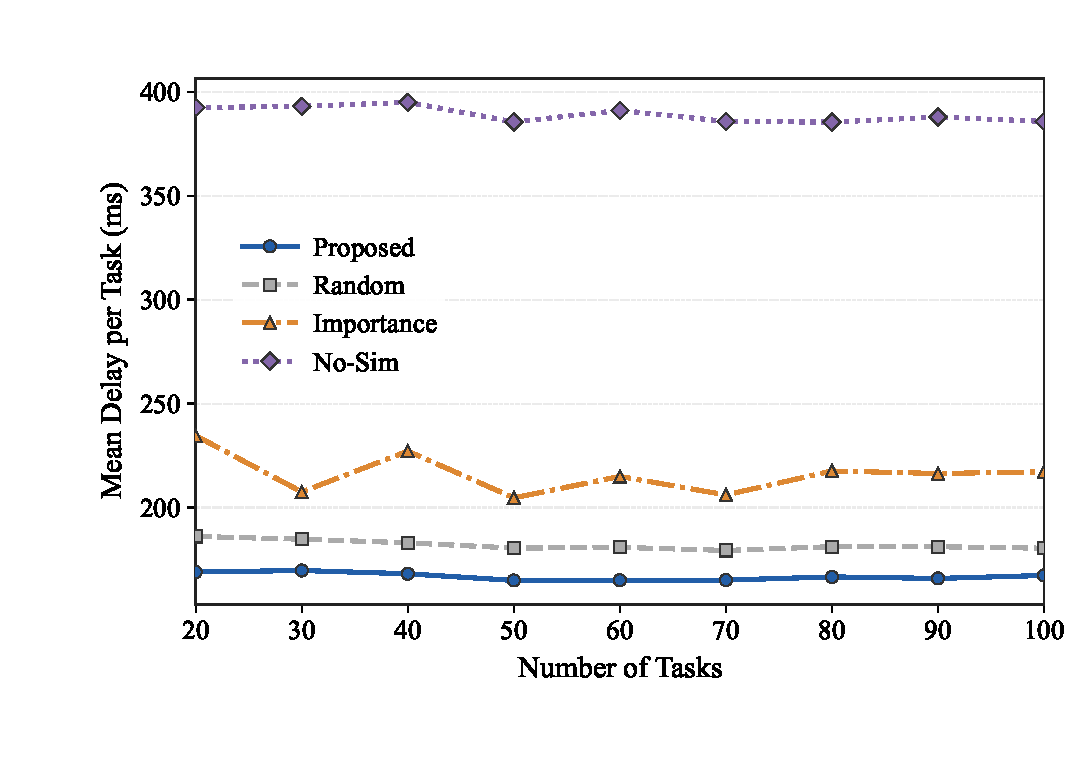
\includegraphics[width=0.98\columnwidth]{fig8_task_count.pdf}%
  }{%
    \fbox{\parbox{0.88\columnwidth}{\centering Missing figure file:\\
    fig8\_task\_count.pdf}}%
  }
  \caption{Average per-task latency as the number of tasks increases.}
  \label{fig:scale_task}
\end{figure}

%Fig.~\ref{fig:scale_expert} 进一步仅增加专家池规模。专家数量增加会扩大候选部署空间，也会加重内存竞争。Proposed 在 8--24 个专家范围内保持最低任务延迟和最高可行性，这是因为相似候选构造将新增专家转化为可替代资源，而动态冗余惩罚避免把有限内存浪费在功能高度重叠的位置上。相比之下，Random 和 Importance 在专家数量较大时更容易产生低收益部署，导致延迟升高并在大规模专家池下波动更明显。No-Sim 不使用替代专家，因此随着专家池变大，它反而更容易受到原始专家覆盖约束影响，在 22 和 24 个专家附近出现不可行。图中 Proposed 曲线随专家数量增加只缓慢上升，说明相似候选构造和冗余惩罚能够缓解专家池扩大带来的内存竞争。
Fig.~\ref{fig:scale_expert} shows the results when increasing the expert pool size from 8 to 24 while fixing the number of UAVs and tasks. A larger expert pool expands the candidate deployment space but also intensifies memory competition. The Proposed scheme maintains the lowest latency and highest feasibility across the entire range, because similarity-based candidate construction converts newly added experts into usable substitutes, while the dynamic redundancy penalty prevents limited memory from being wasted on functionally overlapping placements. In contrast, Random Placement and Importance are more prone to low-gain deployments as the expert pool grows, leading to increased latency and larger fluctuations. No-Sim, which cannot exploit substitute experts, becomes increasingly constrained by original expert coverage requirements and even encounters infeasible cases near 22 and 24 experts. The Proposed curve rises only gradually with expert pool size, confirming that similarity-aware candidate construction and redundancy control effectively mitigate the memory contention caused by a larger expert set.

\begin{figure}[!t]
  \centering
  \IfFileExists{fig9_expert_count.pdf}{%
    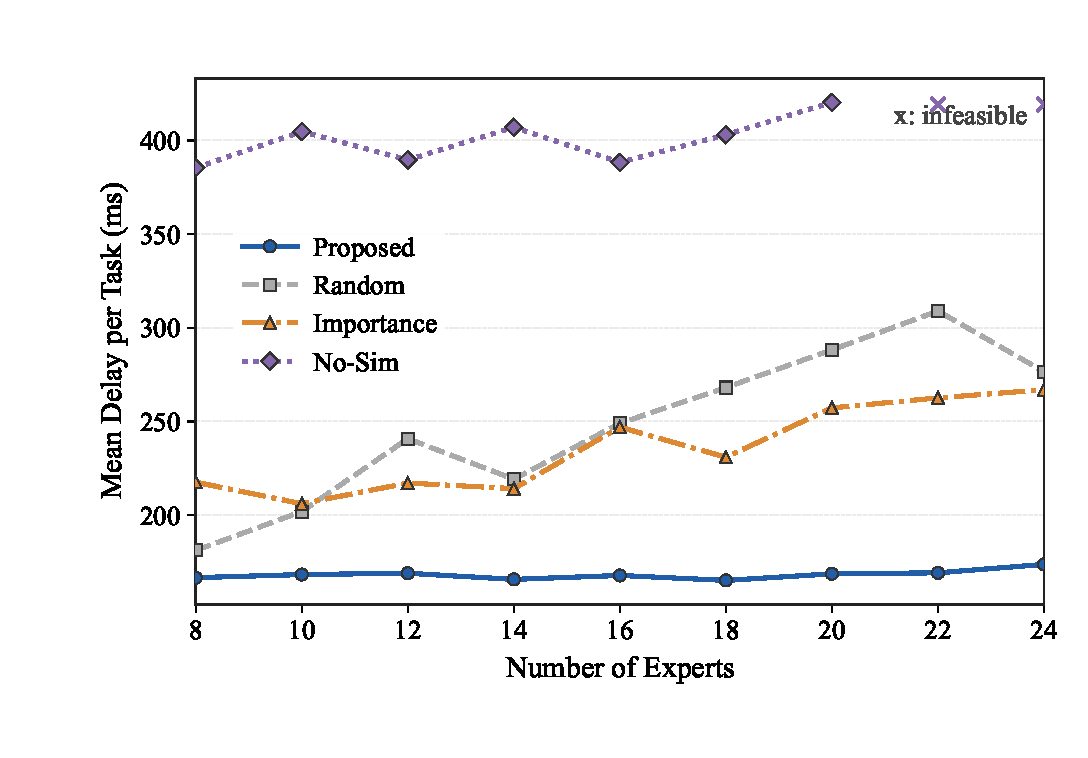
\includegraphics[width=0.98\columnwidth]{fig9_expert_count.pdf}%
  }{%
    \fbox{\parbox{0.88\columnwidth}{\centering Missing figure file:\\
    fig9\_expert\_count.pdf}}%
  }
  \caption{Scalability with respect to expert pool size.}
  \label{fig:scale_expert}
\end{figure}

%总体来看，仿真实验验证了第~\ref{sec:design}~节的核心设计：相似候选构造扩展了可部署专家空间，通信感知评分改善了专家与 UAV 的匹配，动态冗余贪心在内存约束下避免功能重复部署，而轻量级逐层调度将部署结果转化为更低的端到端推理延迟。扩展性实验进一步说明，AeroMoE 在 UAV、任务和专家规模增加时能够保持稳定优势。

% ==============================================================

\section{Conclusion}
\label{sec:conclusion}
% ==============================================================

% 本文研究了 UAV 边缘网络中的 MoE 协同推理问题，重点关注在 UAV 内存、计算能力和单跳通信链路受限的条件下，如何进行专家级部署与推理调度以降低端到端延迟。针对直接部署原始专家容易造成内存压力、忽略通信拓扑又会增加跨 UAV 传输开销的问题，本文提出 AeroMoE，将专家相似性、任务需求、
% UAV 资源约束和通信关系共同纳入部署决策。

% AeroMoE 首先根据任务分布统计各 UAV 区域的专家需求，并基于专家相似度构造可替代专家集合；随后设计通信感知的专家部署评分，并采用两阶段动态贪心策略完成专家部署，其中预部署阶段保证必要专家需求可服务，动态调整阶段在剩余内存中选择收益更高、冗余更低的专家部署方案。最后，AeroMoE根据部署结果执行轻量级逐层调度，为每个专家执行步骤选择本地或单跳可达的UAV。

% 仿真实验结果表明，在本文设置的随机热点 UAV 场景中，AeroMoE 相比Random Placement、Importance 和 No-Sim分别降低了约 $24.1\%$、$21.1\%$ 和 $48.3\%$ 的平均端到端推理延迟。结果说明，相似专家替代能够缓解内存受限下的专家覆盖压力，通信感知部署能够减少不必要的跨 UAV 传输，从而提升 UAV 边缘 MoE 协同推理效率。

This paper addressed the problem of collaborative MoE inference in UAV edge networks under stringent constraints on memory, computation, and communication. We proposed AeroMoE, a similarity-aware framework that integrates expert substitutability, task demand, UAV resource heterogeneity, and communication topology into a unified deployment and scheduling solution. Through extensive simulations in random hotspot UAV scenarios, AeroMoE achieved average end-to-end latency reductions of 24.1\%, 21.1\%, and 48.3\% compared with random placement, importance-based placement, and similarity-agnostic deployment, respectively. These results demonstrate that jointly exploiting expert similarity for candidate expansion and communication-aware placement for topology-aware allocation can significantly improve inference efficiency in resource-constrained aerial edge environments. The proposed approach offers a practical pathway toward deploying large-scale intelligent models on memory-limited UAV platforms without relying on cloud connectivity.

% ---- references ----------------------------------------------
\bibliographystyle{IEEEtran}
\bibliography{IEEEabrv,refs}

\end{CJK*}
\end{document}
